\documentclass[conference]{IEEEtran}
\IEEEoverridecommandlockouts
% The preceding line is only needed to identify funding in the first footnote. If that is unneeded, please comment it out.
\usepackage{cite}
\usepackage{amsmath,amssymb,amsfonts}
\usepackage{algorithmic}
\usepackage{graphicx}
\usepackage{textcomp}
\usepackage{xcolor}
\usepackage{booktabs}
\usepackage{makecell}
\usepackage[most]{tcolorbox}
\def\BibTeX{{\rm B\kern-.05em{\sc i\kern-.025em b}\kern-.08em
    T\kern-.1667em\lower.7ex\hbox{E}\kern-.125emX}}
\begin{document}
\graphicspath{ {./images/} }


\title{Deployment Patterns of Machine Learning Systems: An empirical view} % An empirical view

\author{\IEEEauthorblockN{Dennis Muiruri, Lucy Ellen Lwakatare, Jukka K. Nurminen}
\IEEEauthorblockA{\textit{Computer Science Department} \\
\textit{University of Helsinki}\\
Helsinki, Finland \\
\left\{dennis.muiruri, lucy.lwakatare,jukka.k.nurminen\right\}@helsinki.fi
}}
\and
%\IEEEauthorblockN{2\textsuperscript{nd} Lucy Ellen Lwakatare}
%\IEEEauthorblockA{\textit{Computer Science Department} \\
%\textit{University of Helsinki}\\
%Helsinki, Finland \\
%lucy.lwakatare@helsinki.fi}
% \and
% \IEEEauthorblockN{3\textsuperscript{rd} Jukka K. Nurminen}
% \IEEEauthorblockA{\textit{Computer Science Department} \\
% \textit{University of Helsinki}\\
% Helsinki, Finland \\
% jukka.k.nurminen@helsinki.fi}
\and
\IEEEauthorblockN{Tommi Mikkonen}
\IEEEauthorblockA{\textit{Department of Computer Science} \\
\textit{University of Jyväskylä}\\
Jyväskylä, Finland \\
tommi.mikkonen@jyvaskyla.fi}
}}

\maketitle

\begin{abstract}
%Background and introduction
As machine learning-enabled systems continue to gain adoption, the engineering aspect of these systems has gained increased attention as the apparent complexities continue to surface.
% Objective
This study aims to explore multiple deployment workflows of various ML-enabled systems in the production phase and extract common patterns from the distinct workflows. We consider the deployment process to begin once an ML model has been trained, verified, and accepted for integration in production systems.
%Methods
Using interviews and a multi-case study design, we analyzed eight ML-enabled systems.
%Results
We discuss the following patterns: model versioning and storage, quality assurance, monitoring, model packaging, serving patterns, and inference serving.
%Conclusion
Although ML domains and architectures may differ, commonly adopted practices can serve as a foundation for establishing a standardized ML engineering process.

\end{abstract}

\begin{IEEEkeywords}
deployment, machine learning engineering, machine learning operations
\end{IEEEkeywords}

\section{Introduction}
\label{sec: introduction}
% I
Machine learning (ML) models have increasingly become a part of many software systems in multiple industry sectors as companies seek to provide artificial intelligence (AI) backed services. For example, the healthcare sector has adopted ML methods to improve diagnosis~\cite{sharma2021systematic}, the finance sector has adopted ML approaches to price commodities~\cite{ghoddusi2019machine}, the agricultural industry has developed precision agriculture supported by ML~\cite{9505674}. These and other industries continue to adopt ML~\cite{jan2022artificial} on a wide range of applications. 

Companies tend to begin the adoption of ML applications through experimental initiatives. Once an ML concept is sufficiently explored and validated, the journey begins to transition the model into a production-ready software system. This transition requires significant engineering effort across different stages of the ML lifecycle.~\cite{8498185, lwakatare2019taxonomy}.

% II
The engineering aspect of ML-based software ensures systems are developed, deployed, and maintained efficiently. Practitioners attempt to adopt traditional software engineering practices in ML workflows, but such methods are insufficient or require adaptation to cater to the development process of ML-enabled systems~\cite{amershi2019software}.  
Research on software engineering for ML-based systems is primarily concentrated on challenges experienced during the development process~\cite{8498185, lwakatare2019taxonomy, giray2021software}. Very few studies provide an in-depth review of specific workflow stages, particularly practices carried out after the model training stage, where the model is moved to production systems. Therefore, this presents an opportunity for research that provides empirical evidence that attempts to define high-level standardized procedures. Further, studies that report engineering practices tend to bear the perspective of a single, often large, company whose engineering scale is not comparable to other companies~\cite{amershi2019software, soifer2019deep, Park}. The fundamental reason for the disparity lies in variations across factors such as infrastructure and data availability, research and development capabilities, and investment resources.
%Several studies demonstrating the engineering practices of deploying ML models have been published from a one-company perspective. % reference papers published form FANG

%Other studies focus on the general ML development workflow without providing an in-depth review of the deployment process
% example reference paper https://arxiv.org/abs/2209.09125
% https://dl.acm.org/doi/full/10.1145/3533378

% III
Our study addresses the empirical gap in the deployment of ML models, and in doing so, we make the following contributions. First, we present descriptions of different deployment workflows across various ML domains. Secondly, we synthesize deployment patterns observed at different stages of the deployment workflow: model storage and versioning, quality assurance, monitoring, and model packaging. Third, we also demonstrate varying inference and model-serving architectures.

% IV
Using semi-structured interviews with practitioners to collect data, we probe for detailed issues centred on deployment activities and the processes involved in maintaining the ML-enabled system in production. We use a descriptive case-study approach to characterize the various deployment processes and settings explored in a given interview. As such, we present multiple case studies and inference systems.

% V 
The findings presented in this study will provide a foundation to establish a high-level ML deployment workflow that can be adapted across multiple ML domains. Furthermore, by aggregating diverse inference architectures and deployment procedures, we facilitate an opportunity to compare and evaluate design merits at the early stages of system design. %and applicable practices can be adopted.

% VI (Map of Paper)
This paper is organized as follows: Section~\ref{sec: background and related work} provides background on the deployment of ML models, the scope of deployment activities covered in this paper, and also an overview of previous studies in operationalizing ML-enabled systems. Section~\ref{sec: methodology} presents the research protocol. The results are shown in section~\ref{sec: cases} and~\ref{sec: patterns} as independent case studies and identified patterns, respectively. The obtained results are discussed in section~\ref{sec: discussion}. Section~\ref{sec: validity} provides the validity analysis, while the concluding remarks are presented in section~\ref{sec: conclusion}.



% Background and related work
\section{Background and related work}
\label{sec: background and related work}

Several empirical studies have reported the practices and challenges of ML model\footnote{ML refers to machine learning and deep learning models unless explicitly stated.} development and deployment in industrial settings. The two main distinct phases of the ML workflow ---\textit{training and inference}--- focus on conducting different experiments offline to build an ML model and querying the trained ML model for prediction, respectively. Amershi et.al.~\cite{amershi2019software} presents a nine-stage ML workflow where the last two stages are model deployment and model monitoring. A significant contribution of our work lies in elaborating details of deploying a model as an inference or prediction service, including evaluating various inference architectures across ML domains. This section synthesizes deployment and inference practices based on prior empirical studies. Thus, we focus on expounding the engineering practices applied after an ML model has been trained and selected for deployment.

\subsection{Trained ML model deployment and inference serving}
\label{subsec: trained ML model deployment}
Trained ML models can be deployed on cloud, edge or IoT platforms~\cite{Hazelwood-FB, Wu-FB-edge} and serve millions of inference queries per second daily. Efficient management of inference workloads is paramount to operating and optimizing ML models running in production environments~\cite{Park, Boroumand}. A synthesis of the challenges encountered in deploying ML models across different environments is provided by Chen et al.\cite{Chen}, who analyzed 769 relevant developer posts from Stack Overflow and developed a taxonomy of challenges.

% With many trained ML/DL models across the services, companies typically adopt model serving platforms, such as KServe and Deep Learning Inference Service~\cite{soifer-MS}. Using services available on model serving platforms, developers can upload their trained models on the platforms, often in specified formats (e.g., ONNX/NNEF for DNN models) or invoke platform services to facilitate ML/DL model deployment in production. The backend services of the model serving platform take care of the uploaded trained models and hardware resources to provide a timely, low-latency response to inference requests. Inference requests can then be submitted to the model serving services via an API by the application. Thus, from the developers' perspective, the model-serving platform abstracts the complexity of autoscaling, networking, and server configurations during model deployment. 

% Deployment of the ML/DL models on the server/cloud is the most common approach. The ML-enabled system contacts an API endpoint of the ML/DL models hosted on the server/cloud to access the models. The deployment procedure of an ML/DL model on the server/cloud platform often involves bundling model artefacts into a package (e.g., Docker image\footnote{https://www.docker.com/}), which, when deployed, will run in an encapsulated computing environment/container (uber, Christidis). Openja et al.~\cite{openja} studied how Docker is used in deployment by analyzing 406 open-source ML-enabled software projects. Their~\cite{openja} analysis of Docker image characteristics showed that, compared to traditional software, building ML-enabled applications requires more computation due to the large number of files with deeply nested directories in the image layers.

Deployment of the ML models on the server/cloud is the most common approach, where an API endpoint is provided to query for predictions. Alternative methods are also applied, such as embedding the model into other software components, where the model is accessed through function calls. The deployment procedure often involves packaging model artefacts into a package (e.g., Docker\footnote{https://www.docker.com/} image) and then using deployment platforms such as KServe\footnote{https://www.kubeflow.org/docs/external-add-ons/kserve/kserve/} or Deep Learning Inference Service~\cite{soifer2019deep} to configure and manage the underlying infrastructure resources. A study by Openja et al.~\cite{openja} showed that although Docker improves the portability of models, Docker images require significant computation resources due to many small files and deeply nested directories. Closely related, our previous study~\cite{muiruri2022practices} showed a low adoption and usage of ML serving platforms in small and medium-sized companies, indicating that practitioners at the time preferred simplified deployment workflows.

%ML models can be specifically created and deployed on the edge and Internet of Things (IoT) devices/platforms without relying on the cloud. Typically, constraints related to privacy and connectivity motivate the deployment of ML/DL models on edge devices. However, deploying the ML/DL model at the edge is challenged by the diversity and limitations of the hardware (i.e., compute capabilities) available at the edge, amongst others. Due to performance and memory usage requirements, different ML/DL model size optimization techniques, e.g., quantization and compression, are used. Additionally, specialized edge ML accelerators, such as Google's Edge Tensor Processing Unit and NVIDIA Jetson, are used in a few cases \cite{Wu-FB-edge}. Boroumand et al. \cite{Boroumand} identified several shortcomings of edge accelerators from their study of inference execution of 24 state-of-the-art DL models used in Google mobile applications. The authors' findings suggested that critical components of an edge accelerator (e.g. memory system and data flow) must be co-designed and co-customized based on specific ML/DL model layer characteristics to achieve high utilization and energy efficiency. Wu et al. \cite{Wu-FB-edge} noted that using accelerators on edge is primarily for energy efficiency during execution time, and the speedup is secondary. Three deployment procedures of ML/DL models at the edge can be observed to be in use depending on the application domain and the involved design tradeoffs. The first deployment option involves compiling an application containing ML/DL code to platform-specific object code, leading to a larger model size but smaller interpreter. The second deployment option uses operating system vendor-specific API, e.g., iOS CoreML. The last option involves deploying a generic interpreter, e.g., TFLite.

Deploying ML for edge/IoT applications typically requires the transformation and bundling of the model along with its dependencies for deployment in a specific, optimized environment. This procedure can be approached in various ways, for example, by compiling the ML application to architecture-specific binary, such as a Debian package that can be created and installed on a Linux device. Secondly, using vendor-specific software development kits (SDKs) such as iOS CoreML~\footnote{https://developer.apple.com/documentation/coreml} or using framework-specific tools, such as TFLite\footnote{https://www.tensorflow.org/lite}. Factors such as hardware heterogeneity, support of multiple runtimes, and variance in performance profiles are some factors that can influence deployment workflows in edge and IoT-related environments~\cite{Wu-FB-edge}.

The browser is emerging as another viable ML deployment platform. JavaScript-based frameworks, such as TensorFlow.js and WebDNN, are implemented to support the training and inference of ML models in browsers~\cite{Ma}. Given the browser's limited resources, trained models require an optimization step to ensure they can run within the constraints. Deploying models to the browser environment is relatively more straightforward compared to other platforms~\cite{Chen}.
% For a web application, privacy and real-time response requirements have brought a recent and new trend of performing ML/DL tasks directly on the client side (i.e., using a browser engine to run ML/DL models)~\cite{Goh}. In addition, in-browser ML/DL models help to minimize cross-platform compatibility issues relating to the differences in the underlying hardware (PC, smartphone, wearable) and software (Android, Windows, iOS) ~\cite{Goh}. Various JavaScript-based frameworks, e.g., TensorFlow.js and WebDNN, are implemented to support the training and running of ML/DL models in the browsers \cite{Ma}. Some of the frameworks support the offloading of computation onto a remote server. In-browser ML/DL model deployment and inference involve loading a pre-trained model by downloading a model file from a remote server and getting model outputs with a given input to the model. Like edge deployment, model optimization techniques, like weight quantization, supported by the frameworks, are used to reduce the model size \cite{Goh, Ma}. An empirical study on the feasibility and usability of in-browser DL frameworks showed the need to pre-load the DL model file because the loading process takes longer than the actual inference job \cite{Ma}.

Monitoring is typically performed to track active ML deployments and guarantee the high and accurate performance of the models after the deployment and during inference serving. The performance of ML systems can suffer from data drifts and other drifts in bias and feature attribution (e.g., changes in the relationship between the input and output variable over time)~\cite{Nigenda}. Different metrics are collected, analyzed and interpreted to detect abnormal behaviour, determine their causes and perform corrective measures~\cite{Nigenda}.

\subsection{Related Work}
\label{subsec: related work}
% Intro
%The process of engineering software systems has evolved across several methodologies; an approach such as the waterfall approach preceded agile-based practices before the DevOps approach emerged. The DevOps approach aims to integrate the development and operations functions. This approach supports the continuous integration and delivery of software~\cite{leite2019survey}, ensuring bug fixes and new features are available reliably fast to end users. Introducing ML models to the software ecosystem tends to introduce an added level of complexity to the engineering process. This is mainly due to the added dependency on data, ML algorithms, and models, among other artefacts of the ML lifecycle. Engineering ML-enabled software systems may require a different approach~\cite{ozkaya2020really}. These practices are aimed at ensuring an ML-enabled system can be reliably deployed. Unlike DevOps, which has matured over time, practices to develop ML-enabled systems are still in the early stages of being formed as an established philosophy or standardized process. 

% Subject area: SE4AI, CI/CD for ML
With engineering aspects of ML-enabled systems gaining much attention from researchers recently, most studies have focused on identifying general engineering challenges ~\cite{lwakatare2019taxonomy, paleyes2022challenges, giray2021software, martinez2022software, baier2019challenges} and best practices~\cite{serban}. Our study explores the engineering of ML-enabled systems in varying maturity levels but focuses on identifying standard practices in deploying trained ML models and inference architectures. Paleyes et al. ~\cite{paleyes2022challenges} identify integration, monitoring, and updating of models as sub-steps of the deployment stage. Baier et al.~\cite{baier2019challenges} also distinguish pre-deployment activities from deployment activities where input data, implementation, and infrastructure-related factors are featured. Shankar et al.~\cite{shankar2022operationalizing} cover deployment as part of a broader operations process and indicate that production environments are characterized by the high velocity of experimentation, proactive validation, and maintenance of multiple versions of models. Kolltveit and Li's study~\cite{kolltveit2022operationalizing} focuses on operational activities after model training and evaluation. They outline key aspects of operationalizing ML models: packaging and integration, deployment, serving and inference, and monitoring and logging. Our study takes a similar approach by focusing on activities after a model has been evaluated and ready for inference serving. This way, we provide a deeper insight into integrating the inference code into a targeted environment.
%Software patterns entail reusable solutions to common problems within a given context.  % the rationale of design choices across inference architectures.
Furthermore, our work gives explanation and empirical evidence to studies focusing on understanding general software patterns related to the architecture and design of ML-enabled applications, such as those presented in literature review studies~\cite{washizaki, Lo, heiland2023design} and practitioners' experiences and opinions~\cite{lakshmanan2020machine, take}. Washizaki et al.~\cite{washizaki} summarize and do not elaborate on the listed patterns, and Lo et al.~\cite{Lo} detail patterns for ML systems that apply federated learning. Despite differences in extraction and classification of patterns identified from these studies, examples of patterns presented for the model deployment phase include reusing code between the training pipeline and serving pipeline, decoupling the training pipeline from the production pipeline, event-driven ML microservices, and ML versioning~\cite{washizaki}. %The applicability of well-established patterns to ML systems is explored by Take et al. \cite{take}. Despite differences in the extraction and classification of patterns identified from these studies, our work focuses on providing empirical evidence and explanations for the patterns observed as commonly applied deployment practices and inference architectures applicable in different ML system contexts.

% Baier et al. also make use of 11 semi-structure interviews
% https://link.springer.com/chapter/10.1007/978-3-030-64148-1_12
% https://ieeexplore.ieee.org/abstract/document/10081336

% The context of these two papers
% https://arxiv.org/pdf/2209.09125.pdf (Operationalizing Machine Learning: An Interview Study)
%shizaki ete% https://dl.acm.org/doi/pdf/10.1145/3526073.3527584 Operationalizing Machine Learning Models - A Systematic

\section{Methodology}
\label{sec: methodology}
% Exploratory case studies are used as initial investigations of some phenomena to derive new hypotheses and build theories~\cite{easterbrook2008selecting}
% "A multiple case study offers greater validity"~\cite{easterbrook2008selecting}

% Summary of cases: Business sector, ML domain, Target Platform

\DIFdelbegin %DIFDELCMD < \begin{table}[ht]
%DIFDELCMD <   %%%
\DIFdelendFL \DIFaddbeginFL \begin{table}
  \DIFaddendFL \caption{Summary of ML cases}
    \DIFdelbeginFL %DIFDELCMD < \resizebox{\columnwidth}{!}{
%DIFDELCMD <     \begin{tabular}{lp{2,2cm}p{3cm}p{1.2cm}l} 
%DIFDELCMD <         \textbf{Case} & \textbf{Sector} & \textbf{ML Task} & \textbf{Platform}\\ 
%DIFDELCMD <         \hline
%DIFDELCMD <         1 &  Advertising       & Ad Targeting    & Cloud  \\ % smartly helsinki
%DIFDELCMD <         2 &  Gaming     & Object detection and OCR   & Cloud  \\ % Noice
%DIFDELCMD <         3 &  Healthcare    & Transcription & Cloud  \\ % Inscripta
%DIFDELCMD <         4 &  Financial Services    & Risk Modelling & Cloud  \\ % Aktia
%DIFDELCMD <         5 &  Financial Services    & OCR   & Cloud \\ %Baseware
%DIFDELCMD <         6 &  Software Platform & Multiple ML Tasks & Cloud/IoT \\ % SoftwareAG
%DIFDELCMD <         7 &  Advertising & Ad Optimization  & Cloud \\ % Smartly california
%DIFDELCMD <         8 &  Manufacturing & Anomaly Detection & Edge \\ % Siemens
%DIFDELCMD <         \hline    
%DIFDELCMD <         \end{tabular}
%DIFDELCMD <     }
%DIFDELCMD <   %%%
\DIFdelendFL \DIFaddbeginFL \begin{tabular}{lp{3cm}p{3.5cm}p{2.0cm}p{3.2cm}l} 
        \textbf{\DIFaddFL{Case}} & \textbf{\DIFaddFL{Sector}} & \textbf{\DIFaddFL{ML Task}} & \textbf{\DIFaddFL{Platform}} & \textbf{\DIFaddFL{Interviewee Role}}\\ 
        \hline
        \DIFaddFL{1 }&  \DIFaddFL{Advertising       }& \DIFaddFL{Ad Targeting    }& \DIFaddFL{Cloud }& \DIFaddFL{ML Enginneers (2) }\\ %DIF >  smartly helsinki
        \DIFaddFL{2 }&  \DIFaddFL{Gaming     }& \DIFaddFL{Object detection and OCR   }& \DIFaddFL{Cloud  }& \DIFaddFL{ML Engineers (2) }\\ %DIF >  Noice
        \DIFaddFL{3 }&  \DIFaddFL{Healthcare    }& \DIFaddFL{Transcription }& \DIFaddFL{Cloud  }& \DIFaddFL{CTO}\\ %DIF >  Inscripta
        \DIFaddFL{4 }&  \DIFaddFL{Financial Services    }& \DIFaddFL{Risk Modelling }& \DIFaddFL{Cloud  }& \DIFaddFL{ML Engineer}\\ %DIF >  Aktia
        \DIFaddFL{5 }&  \DIFaddFL{Financial Services    }& \DIFaddFL{OCR   }& \DIFaddFL{Cloud }& \DIFaddFL{Senior Software Engineer}\\ %DIF > Baseware
        \DIFaddFL{6 }&  \DIFaddFL{Software Platform }& \DIFaddFL{Multiple ML Tasks }& \DIFaddFL{Cloud/IoT }& \DIFaddFL{Product Manager}\\ %DIF >  SoftwareAG
        \DIFaddFL{7 }&  \DIFaddFL{Advertising }& \DIFaddFL{Ad Optimization  }& \DIFaddFL{Cloud }& \DIFaddFL{ML Engineer}\\ %DIF >  Smartly california
        \DIFaddFL{8 }&  \DIFaddFL{Manufacturing }& \DIFaddFL{Anomaly Detection }& \DIFaddFL{Edge }& \DIFaddFL{ML Engineer}\\ %DIF >  Siemens
        \hline    
        \end{tabular}
  \DIFaddendFL \label{tab: ml_case_summary}
\end{table}
This study applies an exploratory multiple-case study research design approach \cite{runeson2009guidelines}. The multi-case study research methodology is used because of its suitability in exploring complex phenomena in their real context~\cite{easterbrook2008selecting, runeson2009guidelines}. Ethnographic methods like interviews are a common way to collect data for case studies, especially for studies in software engineering processes~\cite{giray2021software}. We conducted semi-structured interviews with practitioners across eight companies, similar to previous studies~\cite{shankar2022operationalizing, baier2019challenges, lwakatare2019taxonomy}.

\subsection{Research objectives}
As discussed in section~\ref{sec: background and related work}, empirical studies in AI engineering \cite{bosch2021engineering} tend to explore the entire ML workflow and further focus on identifying challenges encountered in various workflow stages. This study specifically focuses on the deployment and inference aspects of the ML/DL model in real-world production settings. That is, considering the process that begins when an ML/DL model is eventually ready for integration into the rest of the software ecosystem. Our goal is to capture patterns of practices applied in converting inference code into an inference service, which is the deployment procedure shown in Figure~\ref{fig:deployment_highlevel_framework}. We interviewed practitioners with hands-on experience deploying ML systems to achieve our objective. A summary of the ML systems, their respective deployment platforms and the case company's business sector is presented in Table~\ref{tab: ml_case_summary}. Our study seeks to answer the following questions:

% Image: an overview of the deployment process
\begin{figure}[h]
\centering
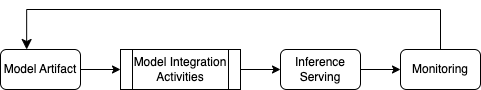
\includegraphics[width=0.5\textwidth]{deployment_highlevel_framework}
\caption{A high-level view of deployment activities}
\label{fig:deployment_highlevel_framework}
\end{figure}

\subsection{Research questions (RQ)}
\begin{itemize}
    \item RQ1) How are deployment workflows of ML/DL models implemented in production settings?
    \item RQ2) What patterns emerge in deployment workflows of ML/DL models?
    \item RQ3) How are inference architectures implemented?
\end{itemize}

\subsection{Case and Participant Selection}
% Unit of analysis?
A case in our multi-case study design approach represents an organization's deployed ML/DL system. By focusing on deployed production systems, we aimed to ensure the interviewee references a tried and tested workflow irrespective of its efficiency. Our goal was to be able to discuss the adopted approaches and, potentially, the rationale of various design decisions.
%The ML code has been deployed into production for an operational software application and service. 

After contacting several companies, we selected companies whose ML-enabled systems had been deployed to production. Three of the companies that responded had participated in our previous study~\cite{muiruri2022practices}, while five cases were new to us. Interviewees in this study were required to be actively involved in deploying the ML system. This was necessary to facilitate a richer discussion on the technology stack choice and potential improvement areas, among other architectural decisions.


\subsection{Data Collection}
Eight semi-structured interviews were conducted, and two researchers were present during the interview sessions. One practitioner from an organization was interviewed, except in one case where two practitioners were involved. The interview sessions were guided by the list of questions in Table~\ref{tab: interview_questions}. These questions were sent to the case companies before the interview. This ensured that the company identified a person with the relevant system knowledge to participate in the discussion. Five company interviews were conducted virtually through video conferencing, and one interview was conducted in a physical meeting, while two companies that were involved in our previous study participated through email correspondence since we were familiar with their solution. All data was gathered between September 2022 and November 2022. All interview discussions were recorded and transcribed for analysis.

Discussions with the interviewees did not strictly follow the order in the list of questions; instead, we probed the interviewee based on the breadth and depth of answers to a given query. Virtual interviews were recorded using zoom\footnote{https://zoom.us/} and transcribed using Otter.ai\footnote{https://otter.ai/}. We manually corrected any transcription errors that appeared before starting the analysis process.

 
\subsection{Data Analysis}
The transcribed text was the primary input for the analysis process. Using the deployment process text descriptions for each case, the two researchers extracted the activities in the deployment process and, at the same time, visualized the inference architecture of the entire ML system. A summary of the deployment process and the inference system architecture were sent via email to each case for validation as well as to get further clarifications. At this phase, researchers initially identified standard practices cross-cutting the cases. 

A systematic cross-case analysis~\cite{seaman1999qualitative} was conducted wherein using our interview questions (rows) and companies (columns), we formed a matrix~\cite{webster2002analyzing} and each response to a question by a given company was extracted, analyzed, and entered into a relevant cell in the matrix. Effectively, the matrix contained eight rows and six columns where a single cell represented a company and its approach to a given topical issue probed with a question. During this analysis process, any conceptual gaps identified in the responses were clarified with the interviewee through email correspondence. We synthesized an overall view for each row and summarised it as a topical deployment pattern.

% Table interview questions

\begin{table}
    %\fontsize{9pt}{8pt}\selectfont
    \caption{Interview Questions}
    \begin{tabular}{p{0.1cm}p{13cm}} 
    \hline
        1 & Can you briefly describe, in a high-level manner, your model deployment procedure? (how do they get models on the edge/cloud server) \\   
        
        2 & What data processing is done for model inference? (Do you perform any parsing or manipulating input data during prediction/inference?) \\
        
        3 & Elaborate in detail the model serving run-time environment, e.g. are you using a custom server, use of containers, use of framework servers (Tensorflow serving) \\
        
        4 & Describe the prediction/inference service, e.g. how is inference served? Batch/realtime/ REST or gRPC-based APIs/in-App Embedded \\
        
        5 & Describe the model update procedure. i.e., where an existing model in production needs to be upgraded, how is model retraining triggered/done post-deployment? \\
        
        6 & Can you describe your deployed model monitoring procedures? e.g. what monitoring metrics are used in production? \\

    \hline    
    \end{tabular}
  \label{tab: interview_questions}
\end{table}



% Image: our data analysis process
\begin{figure*}[h]
\centering
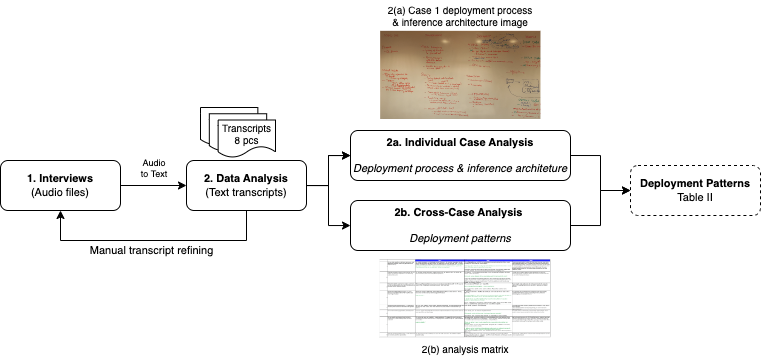
\includegraphics[width=0.9\textwidth]{images/data_analysis_process.png}
\caption{Data analysis process}
\label{fig: data analysis process}
\end{figure*}

%We further depicted each case's inference architecture with a diagram we later sent to the interviewees for validation.

% A straightforward research question concerned with how or why certain phenomena occur
% Case study research uses purposive sampling rather than random sampling


\section{Deployment Workflows and Inference Architectures}
\label{sec: cases}
% A case description has three aspects, the textual description, a diagram, and a table entry. The text description will focus on outlining the processes in a detailed manner while the diagram presents technical/architectural aspects that are best indicated in an annotated diagram than being described. The table entry provides a high-level summary and serves as a comparison tool across the cases.
This section outlines the activities in the deployment procedure of ML models in each studied case. Figure~\ref{fig:deployment_highlevel_framework} summarizes the studied activities in the deployment procedure. For each case, the descriptions provide an overview of the:
\begin{itemize}
    \item ML system use case (or business context)
    \item Integration activities before inference serving, including quality assurance, model packaging, etc. 
    \item Server runtime configurations and server environment setups
    \item Inference service 
    \item Monitoring activities 
\end{itemize}  

%This section outlines the procedure followed in the case study process and a detailed description of each case. The model deployment workflow starts with a validated model artefact produced from the model experiment phase by the model training and testing phase.
%The studied cases are presented in five distinct sections: i) A description of the business context of the ML system, ii) An examination of pre-integration activities, including quality assurance, model packaging, and any other preparations undertaken before inference serving. iii) An examination of server runtime configurations and server environment setups. iv) An examination of serving inference, and finally, v) an analysis of the monitoring activities in place. A comprehensive illustration of this framework is presented in figure~\ref{fig:deployment_highlevel_framework}.


\subsection*{Case 1}\label{1}
% Case Description: Smartly HLK
% deployment setup diagram
\begin{figure*}[b]
\centering
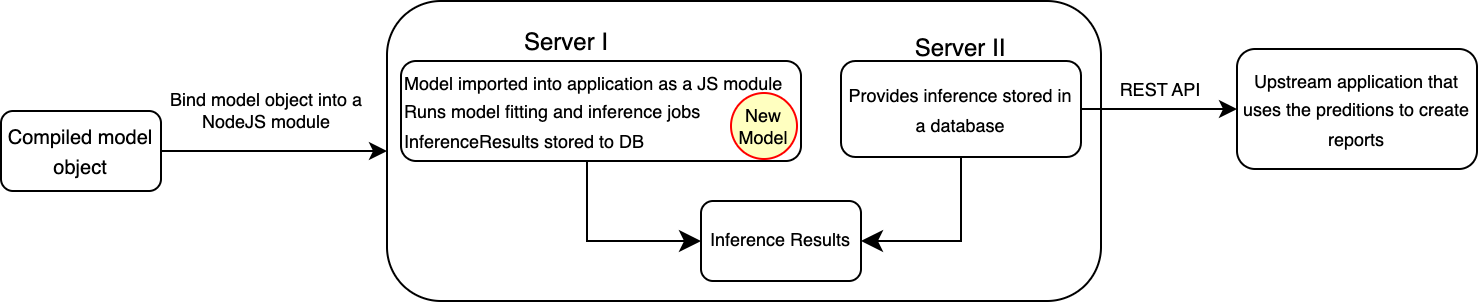
\includegraphics[width=\linewidth]{images/case1_deployment_process.png}
\caption{Case 1 Inference Architecture}
\label{fig: case1_deployment_process}
\end{figure*}

The ML system is part of an advertisement budget allocation system in marketing campaigns. The system uses data from a browsing session context to determine the probability of an Advert viewer converting into a purchaser. The model is built by specifying a STAN\footnote{https //mc-stan.org} program using the STAN\footnote{Stan is a C++ library for Bayesian modelling and Inference that primarily uses the No-U-Turn sampler (NUTS) (Hoffman and Gelman 2012) to obtain posterior simulations given a user-specified model and data.} modelling language. This model differs from typical ML frameworks with distinct fitting/training and inference phases. The model's estimation and Inference occur concurrently in the STAN framework runtime.

\textit{Pre-Integration}: Since no estimated weights and parameters are optimized, a Bayesian model description is compiled into a binary object. The model binary object is packaged as a NodeJS library by binding the model into a nodeJS module. This allows the model to be imported into other Java applications. Updating the model in this setup begins with generating a new version of the code file and re-compiling the file into a new binary object. The business case requires that the model is fitted and new predictions generated daily since consumer behaviour can change drastically, and the Ads should remain highly relevant. To put the scale of operations into perspective, one client can have multiple marketing campaigns, resulting in hundreds of models being updated and used to generate Inference daily.

\textit{Quality assurance}: Quality management is based on performing local tests on the resulting accuracy of the models. These tests are conducted locally and manually orchestrated. The large number of models brings along challenges in identifying faulty models.
% Challenge due to the operations' scale and re-training frequency (Find audio segment reference). This can form part of the discussion topics.

\textit{Server environment}: The deployment setup involves two types of servers: server type I and server type II. Server type I is dedicated to model fitting, generating predictions using the nodes module, and storing the forecasts in a central results database. Server type II is dedicated to serving the prediction results by fetching them from the results database using a REST API. A depiction of this setup is shown in Figure~\ref{fig: case1_deployment_process}. This second server presents the budget allocation service. Batch results are analyzed from this second server daily, and the underlying infrastructure is based on 25 computing nodes. These nodes are separated into a group that performs modelling and inference workloads, while another group is dedicated to providing the inference service API endpoints.

\textit{Inference}: The inference service supports batch and real-time Inference using a REST API that uses JSON to serialize the input and output data. Results from batch inference are stored in an internal data lake accessed by the web server supporting a REST API.

\textit{Monitoring}: Conducted to monitor model accuracy errors and service level errors. Model accuracy is checked through local quick checks, such as the standard deviation of predictions. Due to many models, service level errors are monitored closely because they tend to indicate more significant problems in the system.

% resizing or dedicated page presentation




\subsection*{Case 2}\label{2}
% Case Description: Noice
% deployment setup diagram
\begin{figure*}[b]
\centering
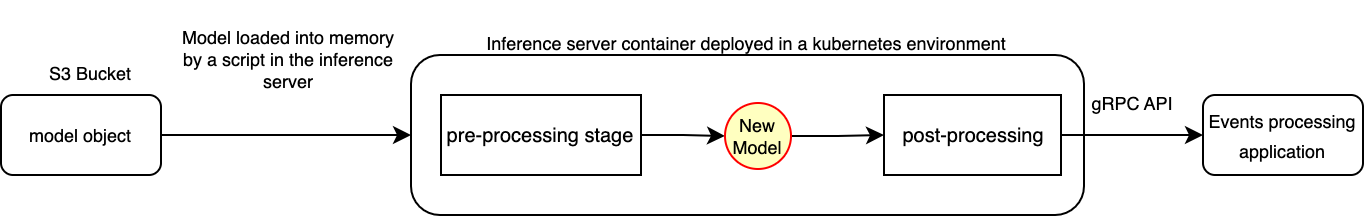
\includegraphics[width=\linewidth]{images/case2_deployment_process.png}
\caption{Case 2 Inference Architecture}
\label{fig: case2_deployment_process}
\end{figure*}

%Case Description: Smartly HLK
%deployment setup diagram
% \begin{figure*}[t]
% \centering
% 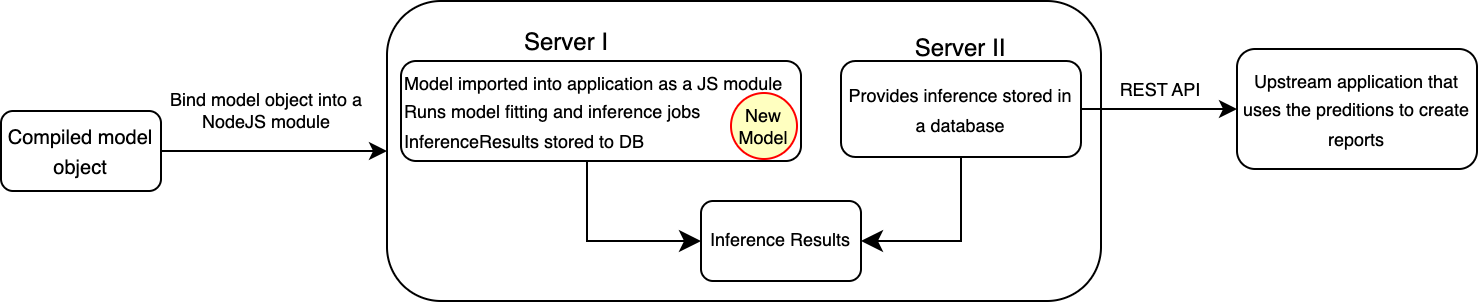
\includegraphics[width=\linewidth]{images/case1_deployment_process.png}
% \caption{Case 1 Inference Architecture}
% \label{fig: case1_deployment_process}
% \end{figure*}

This ML system is a streaming application used to process video streams. The ML system contains a pipeline of two models; an object detection model and an optical character recognition (OCR) model used to process scenes in the video stream. Prediction results from these models are integrated into a solution that seeks to enhance viewer engagement. The system takes a video stream as input data and outputs predicted labels for detected objects and text from video scenes. The solution serves real-time inference to upstream applications that rely on events in the video stream.

\textit{Pre-integration}: The trained models, prepared for deployment, are stored in binary form within an AWS S3 bucket in a designated production folder. The models are manually versioned and typically updated 1-2 times per week, with updates occurring when a newly trained model demonstrates improved offline metrics or new features are added.

\textit{Quality Assurance}: The readiness of a model is assessed through validation using a testing dataset. This involves evaluating several performance aspects of the solution, including collecting performance metrics such as F1 scores, precision, and recall, and testing the real-time inference capability to ensure that predicted events are relevant to the scenes in the video stream.

\textit{Server environment}: The binary files of the two models are loaded into a Docker container. In addition, the preprocessing and postprocessing tasks are encapsulated as functions within a script located in the container containing the model binary. Essentially, the container includes the entire inference pipeline. The model objects are directly accessed within the container, and inference is conducted by loading the loaded model object in memory through a Python script. GPUs are used for the inference process. The predictions are packaged into events as a postprocessing step of the inference procedure using a gRPC-based service for serving prediction results. The Docker images are deployed in a Kubernetes environment, enabling horizontal scaling of the system by running each new video stream in an independent container. % containers are like compute nodes

\textit{Inference}: The video data stream serves as the input to the system, where its frames are periodically sampled for predictions by the model. The inference pipeline involves three steps: (i) a preprocessing step where the frames are resized before being sent to the model for prediction, (ii) a prediction step where the resized frames are supplied to the model for inference, and (iii) a postprocessing step that packages the prediction results into a JSON format which other upstream applications can process. This inference setup is shown in Figure~\ref{fig: case2_deployment_process}. In the prediction step, the model object is accessed directly without using any communication protocol to obtain the predictions. After the postprocessing step, the overall results are served through a gRPC message service.

\textit{Monitoring}:
Monitoring is considered an online activity at the model and business levels. The model level monitoring involves tracking model accuracy using precision, recall, and F1 metrics. Business-level metrics that focus on events in a stream being correctly identified are closely related to the model-level events. The business depends on identifying these events. % The revenue model could be related to the correct identification of events to place Ads



\subsection*{Case 3}\label{3}
Case description: Inscripta 
%deployment setup diagram
\begin{figure*}[b]
\centering
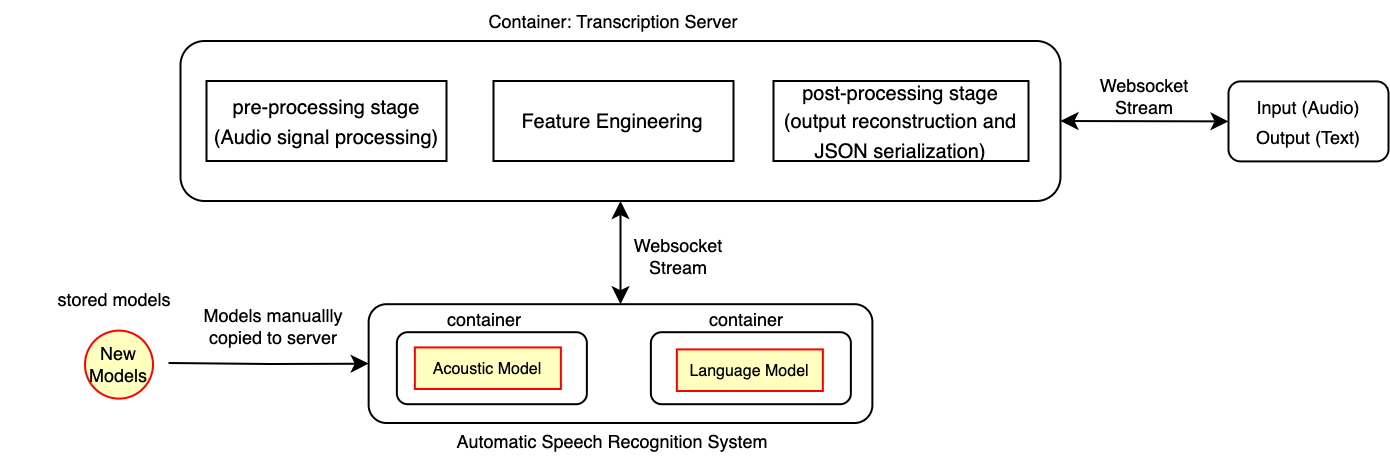
\includegraphics[width=\linewidth]{images/case3_deployment_process.png}
\caption{Case 3 Inference Architecture}
\label{fig: case3_deployment_process}
\end{figure*}

% % Case Description: Noice
% % deployment setup diagram
% \begin{figure*}[t]
% \centering
% 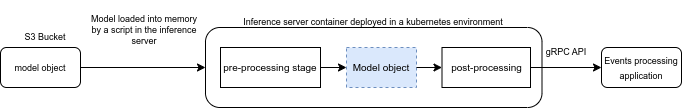
\includegraphics[width=0.8\textwidth]{images/case2_deployment_process_v2.png}
% \caption{Case 2 Inference Architecture}
% \label{fig: case2_deployment_process}
% \end{figure*}

The ML system is an automated speech recognition system designed to transcribe speech data into text for medical and customer service applications. The two applications are based on two distinct models; a medical model trained on medical data and a model trained on business context data. These two types of models are deployed in two independent clusters. However, both systems process streaming speech data and produce transcribed text data. The primary difference lies in the model being deployed. The speech data is collected by a client and streamed to the backend server for transcription. Transcription results are sent to a web application or the client. The transcription service provides a real-time user experience; therefore, the application's performance after deployment is critical.

\textit{Pre-integration}: Trained models are stored in a cloud server and manually copied to the respective inference server with updated configuration files. A rigorous automated CI/CD pipeline ensures high-quality models are deployed, where models undergo testing, building, staging, and production stages. 

\textit{Quality assurance}: The testing phase involves performing local quick checks and unit tests, then building a docker image of the model. An end-to-end and integration test is conducted on the resulting image, and the docker image is deployed to a staging environment for re-testing. A version of the model is approved for deployment to the production environment after all tests have passed. 

\textit{Server environment}: The inference server is versioned, and each version instance contains a unique model version. The server is packaged as a docker image and deployed in a Kubernetes environment, ensuring the deployment can work across multiple vendors. The model in medical deployment is generally stable from a training perspective and serves various medical contexts. On the other hand, the customer service models tend to drift easily, and the deployment contains about 20 model variants. %In general, the deployment architecture is designed to work in multi-vendor settings, and the system comprises two deployment clusters: the medical and the customer service deployment.

\textit{Inference}: The inference pipeline contains similar components across the two deployment clusters (medical and customer service), making it easy to swap models, scale, and replicate the service. Replication supports multiple languages; each language can be scaled according to the number of users. The pipeline contains the following stages: i) a pre-processing step where audio data is converted into raw wave files with a fixed sampling rate, empty sections of the audio file are skipped, and feature extraction algorithms are applied, ii) the transformed data is sent to the ML server through a WebSocket connection, and ii) the inference is converted to JSON format for web applications to use. This pipeline runs in real-time, streaming data to the WebSocket server and presenting the results to the user. This inference architecture is shown in Figure~\ref{fig: case3_deployment_process}.

\textit{Monitoring}: The system is mainly monitored for latency and general availability. Real-time inference is essential for online deployment, and the system must also be highly available to its users. The models are monitored for drift based on customer feedback. In extreme cases where a customer experiences significant degradation in performance, a dedicated model can be provisioned for that customer based on updated training data or other configurations in the model.


\subsection*{Case 4} % Aktia 
\label{case: 4}
% deployment setup diagram
%DIF <  \begin{figure*}[t]
%DIF <  \centering
%DIF <  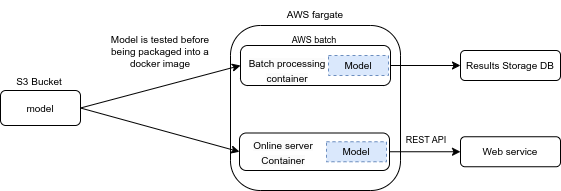
\includegraphics[width=0.8\textwidth]{images/case4_deployment_process_v2.png}
%DIF <  \caption{Case 4 deployment setup}
%DIF <  \label{fig: case4_deployment_process}
%DIF <  \end{figure*}
\DIFdelbegin %DIFDELCMD < 

%DIFDELCMD < %%%
%DIF <  Case description: Inscripta 
%DIF <  deployment setup diagram
\DIFdelend \begin{figure*}[t]
\centering
\DIFdelbeginFL %DIFDELCMD < 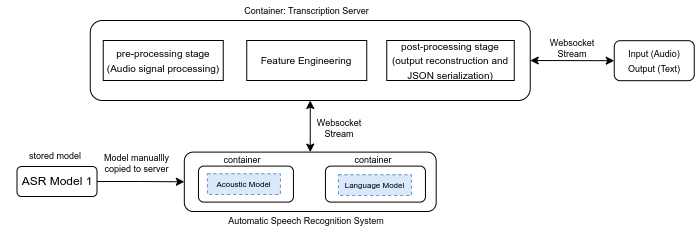
\includegraphics[width=0.8\textwidth]{images/case3_deployment_process_v2.png}
%DIFDELCMD < %%%
\DIFdelendFL \DIFaddbeginFL 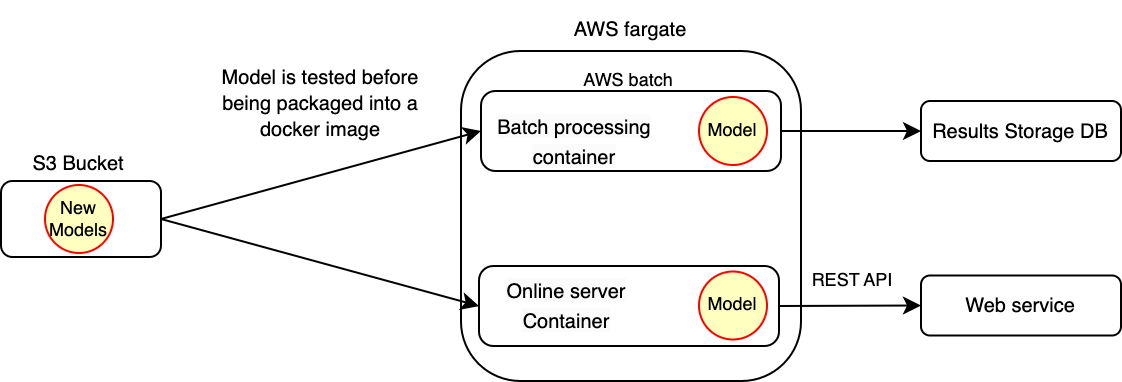
\includegraphics[width=\linewidth]{images/case4_deployment_process.png}
\DIFaddendFL \caption{Case \DIFdelbeginFL \DIFdelFL{3 Inference Architecture}\DIFdelendFL \DIFaddbeginFL \DIFaddFL{4 deployment setup}\DIFaddendFL }
\DIFdelbeginFL %DIFDELCMD < \label{fig: case3_deployment_process}
%DIFDELCMD < %%%
\DIFdelendFL \DIFaddbeginFL \label{fig: case4_deployment_process}
\DIFaddendFL \end{figure*}
\DIFaddbegin 

%DIF >  % Case description: Inscripta 
%DIF >  % deployment setup diagram
%DIF >  \begin{figure*}[t]
%DIF >  \centering
%DIF >  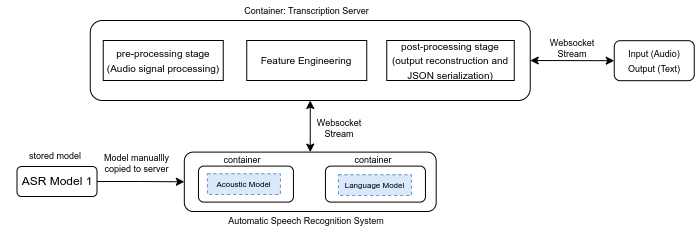
\includegraphics[width=0.8\textwidth]{images/case3_deployment_process_v2.png}
%DIF >  \caption{Case 3 Inference Architecture}
%DIF >  \label{fig: case3_deployment_process}
%DIF >  \end{figure*}
\DIFaddend 

The ML system generates risk classification profiles of clients in financial services setting. This system is part of a broader microservices supporting analytics and predictive risk management services. Financial services are typically regulated, imposing explainability requirements on algorithms and models used to support business process decision-making. The models are trained from data obtained from internal systems. The inference results are stored in an internal datalake accessible to other software components in the broader ecosystem. 

\textit{Pre-integration}: The entire process is centred on a CI/CD pipeline (Atlassian Bamboo) that first involves building the model code into a docker container for the training workflow. The building process is managed with a custom shell or Python scripts. The resulting model artefact moves to a quality assurance stage, which is tested before being serialized and stored in a versioned S3 bucket. Models are updated routinely based on a schedule (weekly, monthly) or based on business demands; the routine updates are based on re-training workflows configured with Airflow.

\textit{Quality assurance}: Other sanity and basic tests are carried out before the model is deployed. This may involve checking metrics (MAE, RMSE) or resulting data distributions.
The versioned storage allows tracking changes in the model artefact to increase the traceability of models due to regulatory demands. 

\textit{Server environment}: A model is deployed in two configurations: i) batch inference processing and ii) as an online prediction service. The batch deployment uses AWS batch and AWS Fargate services to run the batch inference jobs. AWS batch provides the scheduling functionality, while the AWS Fargate provides a serverless container computing environment. The online prediction model is a containerized Python-based server. 

\textit{Inference}: Batch inference jobs are executed regularly on a weekly or monthly basis to generate predictions using pre-processed input data stored in a data lake, and the inference results are stored back into the data lake. The process involves direct access (through function calls) to a serialized model object without using web-based endpoints.
Online inference, on the other hand, is performed through a REST API endpoint that provides real-time predictions to users. This is achieved by sending requests to the API endpoint and receiving immediate responses. This inference architecture is shown in Figure~\ref{fig: case4_deployment_process}.

\textit{Monitoring}: The monitoring setup includes an API gateway to monitor and secure the real-time endpoint and a dashboard that aggregates model metrics such as drift. In addition, other monitoring aspects are handled using Splunk, including monitoring batch run’s success/failure and responsiveness of live endpoint runs, among others.

\subsection*{Case 5} % Baseware 
\label{case: 5} 
% Inference architecture
% \begin{figure*}[t]
% \centering
% 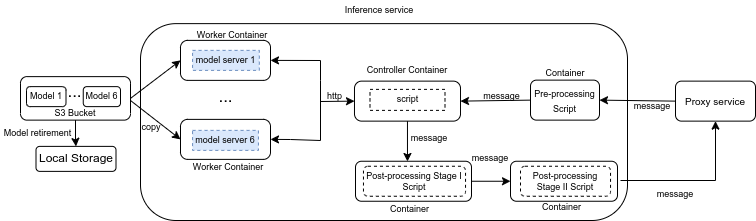
\includegraphics[width=0.8\textwidth]{images/case5_deployment_process_v2.png}
% \caption{Case 5 deployment setup}
% \label{fig: case5_deployment_process}
% \end{figure*}

% deployment setup diagram
\begin{figure*}[t]
\centering
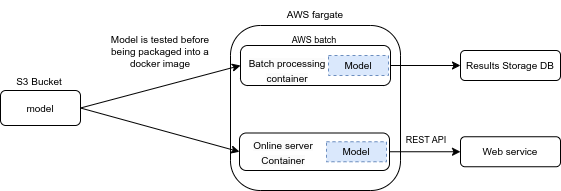
\includegraphics[width=0.8\textwidth]{images/case4_deployment_process_v2.png}
\caption{Case 4 Inference Architecture}
\label{fig: case4_deployment_process}
\end{figure*}

The case company provides electronic invoice management solutions facilitating invoice data exchange. The AI system is a part of this solution. It mainly extracts data fields from a PDF invoice and converts them into text format, which the user can submit to electronic invoice processing systems. Underlying the AI system is an optical character recognition model that uses a combination of NN techniques to extract and predict an invoice’s text field. This system levels the field for SMEs that still use PDF invoices, but the model must handle many unseen PDF layouts during inference.


\textit{Pre-Deployment}: The ML system consists of 6 models (approx. 350MB each) that provide inference concurrently, and each model is trained on a subset of the dataset. Multiple models are designed to improve confidence in the overall prediction results through a voting mechanism. One version of each model is stored in an S3 bucket where other components of the inference architecture access the model. As a retirement policy, once a model is considered for retirement from production, it is stored in an offline server while the online version is deleted from the inference server.

\textit{Quality assurance}: The deployment workflow includes a CI/CD (Bamboo) pipeline with staging and production environments in a cloud setting. The quality assurance process begins with performing local tests on each model by running inference on a dataset of around 1000 documents. These local tests serve as the acceptance tests, and models that pass these tests proceed to the staging environment, where integration and regression testing occurs. Coverage and accuracy metrics are collected at this stage to determine whether the models meet the required quality standards for moving to the production stage. Once in the production environment, an additional testing step is performed using around 20 documents to ensure the model remains functional.

\textit{Server Environment}: The model binary is packaged into a docker container where it is directly accessed during inference. The inference service contains multiple components in a micro-service architecture, including data processing containers, a controller container, and six worker containers that generate inferences. The elements communicate through a messaging queue service (AWS Messaging), but the controller container communicates with the worker containers using HTTP. The data processing and the controller docker containers run scripts (no server), but the worker nodes are Python-based server containers. The controller node distributes inference jobs to the six independent worker servers, which carry out the predictions and return results to the controller node. The architecture is generally designed as a serverless setup using scripts to perform tasks and a messaging protocol to communicate across components.

% Re-Write the inference section a bit to introduce the inference pipeline
\textit{Inference}: To perform inference, a proxy service typically submits a request to an input queue specifying the location of the documents needing processing. The system then pre-processes these documents and generates predictions on various form fields. These predictions are submitted to an output message queue in JSON format. The proxy service can retrieve the predicted results from the output queue for further use. This process is typically performed in a batch mode for more optimal inference processing.

As shown in Figure~\ref{fig: case5_deployment_process}, the inference pipeline is a modular sub-system composed of containerized scripts and a server that performs inference. This setup is optimal for scaling at the sub-process level. The first set of containers (data generators) download a document in PDF format, extract data from it, and transform the data into an array of characters per document. These obtained data objects are then packaged in JSON format and submitted to a queue where the next container in the pipeline ("the batcher") collects and batches several records, effectively processing multiple documents. The batching container stores the batch of character arrays in an S3 bucket in JSON format. 

The next component of the pipeline is a container (controller) that fetches the batched data from the S3 bucket, transforms the data into Numpy arrays, and then submits the data to the models for inference through HTTP requests. There are six models, each in a server container(worker) that produces inference and responds to the controller container when the inference has been completed. A given worker container fetches the array of characters from the S3 bucket and converts them to Numpy arrays before submitting them to the model for inference. The worker further transforms obtained predictions from Numpy arrays to JSON arrays stored in the S3 bucket. After the successful execution of the inference process, a worker reports to the controller, and the controller sends a message to a queue where the next container (extractor) in the pipeline will post-process the results.

Post-processing of the results involves conducting heuristics and local basic checks to determine the quality of inference results. At this stage, the results are also automatically or manually validated based on the threshold of defined accuracy. This process is completed by sending batch results to a message queue where the final component of the pipeline will fetch the results. %(audio segment 49:00).

The final component in the pipeline is also a containerized script that de-batches the results into independent results per document, followed by performing any necessary transformations of the results before submitting them into the final queue where the proxy service fetches results.

\textit{Monitoring}: Monitoring involves checking the system's general availability. Splunk collects logs, monitors resources, and sends alerts in case of a service outage. The coverage metric is calculated by comparing the proportion of documents with confidently accurate inference results to those requiring human validation to confirm their inference results. If the ratio of documents that need human validation increases, it can indicate a decrease in coverage and potentially degrading model performance.
\subsection*{Case 6} % SoftwareAG 
\label{case: 6}
% Inference architecture
\begin{figure*}[b]
\centering
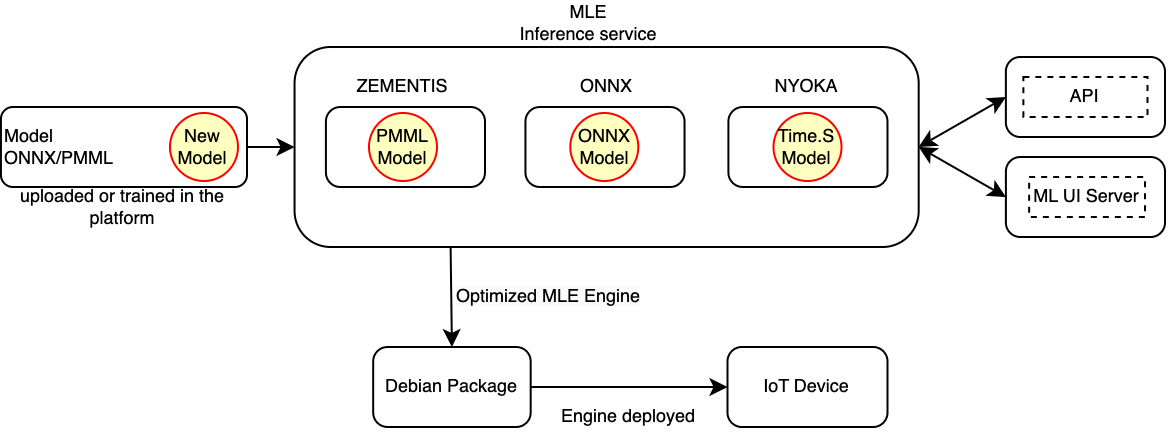
\includegraphics[width=\linewidth]{images/case6_deployment_process.png}
\caption{Case 6 deployment setup}
\label{fig: case6_deployment_process}
\end{figure*}

% Inference architecture
% \begin{figure*}[t]
% \centering
% 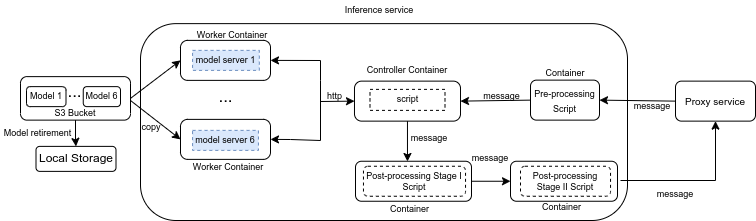
\includegraphics[width=0.9\textwidth]{images/case5_deployment_process_v2.png}
% \caption{Case 5 Inference Architecture}
% \label{fig: case5_deployment_process}
% \end{figure*}

This case company develops an IoT fleet management platform that provides control, monitoring, analytics, and ML functionality for retrofitted or inbuilt sensors. We focused on the ML component of the platform, which offers model management, model training, and model deployment functionality. These functionalities are embedded in two modules: the machine learning workbench (MLW) and the machine learning engine (MLE), respectively. The MLE system handles deployment-related tasks. The entire ML system is accessible through a web interface to support low-code use cases and an API for programmable use cases. Each sub-module can be used independently, allowing users to adopt only the desired functionality and alternative external tools for other aspects of their ML workflow. The use of native Python scripts and Jupyter Notebooks are also supported for more programming-oriented users, which allows the use of more advanced modelling approaches, such as using neural networks. The entire platform is accessible through a web interface or a REST API. %The ML system contains multiple inbuilt time-series analysis algorithms that provide an autoML capability.

\textit{Pre-Deployment}: Models can be added to the platform in two ways: they can either be trained on the platform or uploaded as pre-trained models. However, these models need to be packaged in either PMML (Predictive Model Markup Language) or ONNX (Open Neural Network Exchange) formats which facilitate ML framework and hardware-agnostic deployments. Models are stored on the platform with no elaborate versioning mechanism. Instead, version management is implemented at the project level, where various artefacts belong to a given project. Models can be in one of two states: active or inactive. An active model is kept in memory, while an inactive model is stored in a colder location and removed from memory. It is also possible to delete a model entirely if desired. If multiple model versions are needed, they can be stored as a model group, allowing the models to be managed together. 

\textit{Quality Assurance}: During the model import and conversion process, the platform has a parser that checks the uploaded model's file for semantic errors and makes automatic corrections. Some parsing errors still require manual resolution. The system’s workflow does not include quality assurance steps or integrations. Such would need to be handled outside of the system. %

\textit{Server Environment}: The MLE, the platform's inference engine, handles deployment-related functions. The system is composed of four main microservices: i) zementis, which serves and manages PMML-based models; ii) ONNX, which serves and manages ONNX-based models; iii) nyoka, which provides time-series and clustering models; iv) machine-learning, a web user interface that provides interaction points to the rest of the micro-services. These components are shown in Figure~\ref{fig: case6_deployment_process}. A programmatic interaction with the MLE system is also available as an API, allowing greater flexibility and facilitating integration with other systems.

Since MLE and the rest of the components are provided as a hosted platform, other low-level issues related to infrastructure provisioning, virtualization, runtime, and application containerization are eliminated from the developer’s workflow.

For IoT deployment, the platform generates an optimized version of the MLE runtime as a Debian package. This package is installed on the target IoT devices and the model artefacts for inference.

\textit{Inference}: The platform supports online and batch inference through REST APIs. In batch inference scenarios, the input size is limited to 500MB, and results are returned as a compressed zip file. 

ONNX models support more complex inference workflows by having inference pipeline objects which consist of pre/post-processing steps and inference. The pre/post-processing steps are implemented as scripts, and the inference results are packaged into JSON format. For example, such a process is used in an edge computer vision task.

By default, a model trained in the platform is deployed to the MLE engine, considered a cloud deployment. Inference can be carried out through an API call or the web interface. Models deployed to IoT or edge devices provide inference using the runtime’s command line tool directly on the device.

%The platform provides an API to generate a time series model for inference. This process is implemented as an asynchronous call that returns a status URL which the calling entity can periodically query for the model's status. The model can provide inference from the cloud (MLE) engine or be downloaded and installed on an edge device.

\textit{Monitoring}: The platform provides an API to access a model’s memory footprint and prediction scoring metrics. The scoring metrics are cumulative of the various versions of the model and only available for classification and regression models.
\subsection*{Case 7} % smartly california (viralspace.ai)
\label{case: 7}

% Inference architecture
\begin{figure*}[b]
\centering
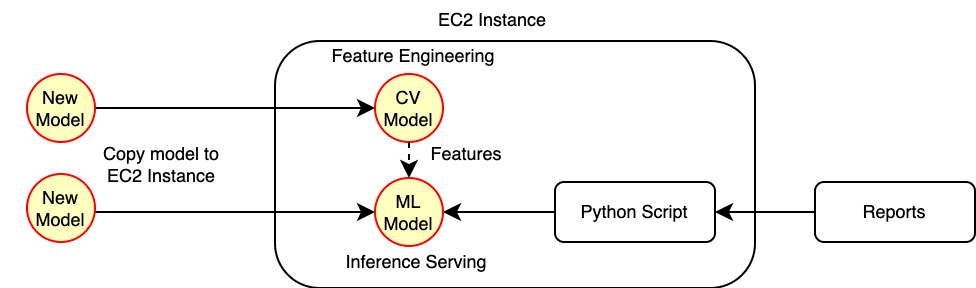
\includegraphics[width=\linewidth]{images/case7_deployment_process.png}
\caption{Case 7 deployment setup}
\label{fig: case7_deployment_process}
\end{figure*}

% Inference architecture
% \begin{figure*}[t]
% \centering
% 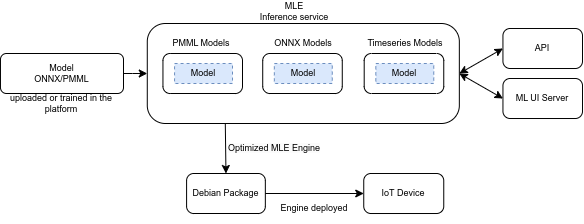
\includegraphics[width=0.9\textwidth]{images/case6_deployment_process_v2.png}
% \caption{Case 6 Inference Architecture}
% \label{fig: case6_deployment_process}
% \end{figure*}

The case company offers an ML system that generates targeted digital advertisements by optimizing the creative elements of ads and suggesting features that can enhance a brand's marketing campaign. The system can also be used to predict an advert's performance before the start of a campaign. The ML solution is comprised of two ML subsystems: i) a computer vision model used for feature engineering tasks such as extracting features from image or video data and performing tagging and labelling, ii) an ML model (non-neural network) that is trained using the features extracted by the CV model. The second model is employed to draw inferences for the business case. These ML models are used internally to generate non-technical reports. As such, customers do not interact with the models directly. % by estimating key performance metrics such as cost per acquisition.

\textit{Pre-Integration}: Generally, the infrastructure is based on AWS services. EC2 instances are used to perform training and inference tasks, while S3 buckets are used to store trained models. The deployment workflow is manually orchestrated. Various elements in the workflow are orchestrated through Python scripts and manual interventions. Each customer is associated with a dedicated model, and the operation's scale involves tens of models, adding to the pipelines' complexity and the general workflows.

Active models are retrained daily to ensure the model accounts for new data obtained from the campaigns. This involves about 100MBs – 1GB of new data depending on the marketing campaign size. The CV model is retrained monthly since it only extracts features from videos and images. The versioning of the models is based on the S3 storage policy, which works as the model retirement policy.

\textit{Quality assurance}: The quality assurance process is centered around a human-in-the-loop workflow. Before deployment, a human reviewer locally validates the performance of a new model to ensure that it meets the required metrics, such as F1-score, or ensures the accuracy of the CV model used for tagging and labelling images is acceptable.

Various factors trigger the model's retraining: new incoming data, new labels from clients for a particular feature, or new Ads being pushed by customers previously unseen by the models.

\textit{Server Environment}: The models and related runtime dependencies to the models are installed into an EC2 instance. No wrapping containers or virtual machines are used in this setting. Instead, Python scripts load models into the instance's memory and from where other components access the models.

The EC2 instance runtime is configured using bash script templates, and the same scripts can be used to create a local runtime environment for development purposes. The runtimes can be used for inference machines or other data exploration tasks. Although the environment is not containerized, the scripts provide a flexible template for managing the runtime environment and adapting it to various needs in the workflow.

\textit{Inference}: The inference pipeline is automated using AWS Lambda. The model object is loaded into the instance's memory, and batch inference is conducted using a Python script. The inference results are then persisted in a database for subsequent report generation. Lambda execution environment offers automatic scaling capabilities which support inference across multiple models and in a single model. Figure~\ref{fig: case7_deployment_process} presents an architectural view of this setup.

Inference for the CV model is used as part of feature engineering and data pre-processing. Pre-processing tasks such as tagging, labelling, encoding strings, and converting them into a vector space are conducted with the CV model.

\textit{Monitoring}: Monitoring begins with ensuring the model's availability using the AWS CloudWatch service. However, logging is the primary method for collecting lower-level information about processes and system events. Other tools such as Lambda, Slack, Email, and Pager Duty are integrated into the monitoring workflow to process events and logs. Given the complex nature of the system, which comprises multiple models, monitoring can become challenging, particularly with the diversity of alerts generated across various channels.

% Inference architecture
% \begin{figure*}[ht!]
% \centering
% 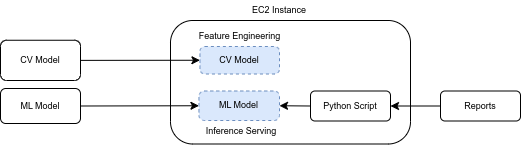
\includegraphics[width=0.8\textwidth]{images/case7_deployment_process_v2.png}
% \caption{Case 7 Inference Architecture}
% \label{fig: case7_deployment_process}
% \end{figure*}

\subsection*{Case 8} % Siemens
\label{case: 8}

% Inference architecture
\begin{figure*}[b]
\centering
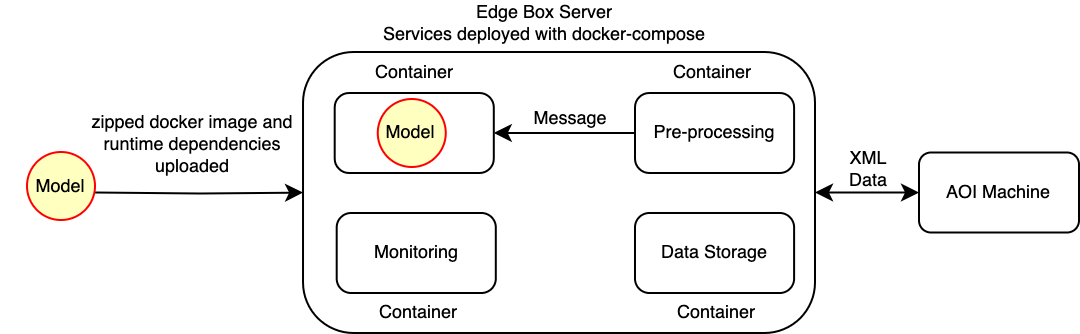
\includegraphics[width=\linewidth]{images/case8_deployment_process.png}
\caption{Case 8 deployment setup}
\label{fig: case8_deployment_process}
\end{figure*}
% Update the image if a post-processing container is missing or confirm how post-processing is handled

% Inference architecture
% \begin{figure*}[h!]
% \centering
% 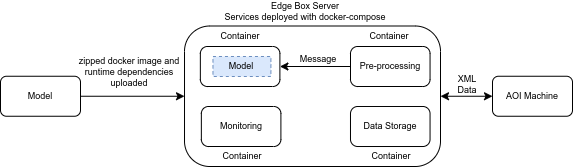
\includegraphics[width=0.8\textwidth]{images/case8_deployment_process_v2.png}
% \caption{Case 8 Inference Architecture}
% \label{fig: case8_deployment_process}
% \end{figure*}

The case company is a manufacturing enterprise that produces industrial and consumer electronic devices. The ML system discussed in this case is mainly applied as part of a quality inspection process on an electronics manufacturing production line. The quality control process has an automated optical inspection (AOI) machine that classifies the manufactured products as defective or non-defective. This process tends to generate a significant number of false negatives. The ML system complements the quality control process by determining whether the manufactured artefact is defective before the product is inspected. The ML system improved the manufacturing process by reducing the effort required for manual inspection. The ML-based process is also designed to ensure that false positives remain minimal. Data used to train the ML model is obtained from the AOI machine in XML format, and labelling occurs during the manual inspection. The resulting ML system is deployed in an edge server (edge box) not connected to the internet.
 
%Data preprocessing begins by parsing the XML data into a tabular format and applying a Scikit-learn pipeline for scaling and classification. The same preprocessing pipeline used during training is also used during inference to ensure consistency and accuracy. 

\textit{Pre-Integration}The entire ML workflow is mainly conducted within the context of DVC\footnote{https://dvc.org/} pipelines. The pipeline is configured around two workflow stages: i) data preprocessing (parsing to tabular form, scaling) and ii) model training, tuning, and evaluation, and saving a versioned model. This pipeline can be run locally or in an AWS EC2 instance. The resulting artefacts (model, reports, images, etc.) are stored in DVC-integrated remote storage connected to an AWS S3 bucket. Versioning of models is manually implemented through git tags.

\textit{Quality assurance}: Quality assurance is based on a CI/CD pipeline that runs after the model has been versioned and committed to DVC for storage. At this stage, tests are carried out at the code level (unit test) and system level, including testing the DVC pipeline and end-to-end tests.

\textit{Server Environment}: The serialized model file is copied to a docker container, and this container, among others, is run on a designated server (edge box). Transferring the containerized server and other containers to the edge server is done by uploading a zip to an edge server through an edge management system. The zip file contains the necessary runtime libraries, config files, docker-compose files for orchestrating container deployments, the model binary, and the application code. This offline deployment arrangement is required because the edge box is not connected to the internet.

The deployed solution involves multiple containers dedicated to a given task, such as receiving and preprocessing data, storing the data, running the model, and monitoring the dashboard. This setup is contained in a docker-compose configuration file. Communication between various containers is based on the MQTT protocol. 

\textit{Inference}: The AOI machine has an in-built computer that generates XML data stored in a file share location for retrieval by other applications. This data performs the anomaly detection task through an inference pipeline. The inference pipeline has three steps i) a preprocessing step where parsing of XML data to tabular takes place. ii) a prediction step where the model is queried for prediction and iii) a post-processing stage where the prediction results are parsed back to XML format. Figure~\ref{fig: case8_deployment_process} shows an architectural view of this setup. This system is integrated into the manufacturing process, where the ML inference process is constrained to complete within 10 seconds before the AOI machine receives another item to process.

\textit{Monitoring}: The overall setup monitoring is undertaken with the edge management system, which shows high-level metrics indicating the health of the containers. The parameters of the AOI machine can change, causing drift which requires a new model to be trained and deployed. Such drift is detected from changes in performance metrics.

% Table summary of cases
\begin{table*}[ht!]
\fontsize{7pt}{8pt}\selectfont
\renewcommand{\arraystretch}{1}
\renewcommand{\cellalign}{vh}
\renewcommand{\theadalign}{cc}

 \centering
  \caption{Summary of cases}
  \begin{tabular}{p{0.6cm}p{3.2cm}p{2.5cm}p{3.2cm}p{3cm}p{3cm}}      
    \toprule
    \thead{Case} & \thead{Pre-Integration} & \thead{Quality\\ Assurance} & \thead{Server\\ Environment} &\thead{Inference} & \thead{Monitoring}\\
    \toprule \\
    1 & Model description (Bayesian) is compiled into a binary object wrapped in a library. 
    Model versioning is dependent on code versioning. The model description does not require regular updates & Local sanity checks on model accuracy & Two server types: one dedicated to model fitting and inference and other servers dedicated to serving from the database Infrastructure is based on 25 compute nodes shared between the two server types & Inference is served through a REST API and data transferred in JSON format & Model accuracy and service level errors \\
    \midrule[0.01pt]
    2 & Solution contains two distinct models working together in a pipeline. Models are stored in AWS S3 buckets as binary objects. Model versioning is manually managed and updated weekly or when a new model is available & Collection of model performance metrics (e.g. precision) from a validation dataset. Check inference latency & Both models are packaged in the same docker container. Preprocessing and postprocessing functions are also in the same container. & An inference pipeline with pre and post-processing stages. gRPC protocol used to serve real-time predictions & Online monitoring of model performance metrics. Business-level metrics that involve correctly identified events in a stream. \\
    \midrule[0.01pt]

    3 & Solution contains two models applied to two different business cases. The models are stored in a cloud server. & Follows a comprehensive automated CI/CD approach. Sanity checks, unit tests, integration, and end-to-end tests are conducted & The two models are deployed into independent clusters. Docker containers are used to package servers and other services of the microservice & Implemented as an inference pipeline where the pre-processing and post-processing steps are detached from the inference server & Latency and availability aspects. \\
    \midrule[0.01pt]

    4 & Solution is based on a single model trained and stored in an S3 bucket where versioning is activated. Model versioning is managed by the bucket and updated on a scheduled routine & An automated CI/CD pipeline is used from the training to creating a deployment model. Sanity checks and basic tests are applied & The model and Python scripts are packaged into a docker container. & Provides batch and online inference. Serverless technologies are used to provide batch service. Online inference based on REST API & Scheduled batch runs. Availability of the online model. Model drift \\
    \midrule[0.01pt]

    5 & ML system contains six replicas of a model. Each model has a version of it stored in an S3 bucket. Models are updated 2-3 times a year, and retired models are stored locally & The process follows a CI/CD pipeline with staging and production environments. Locally conducted tests serve as acceptance criteria. Coverage and accuracy metrics are key model quality assessments & Each model binary is packaged in a docker container. Other components/scripts in the architecture are also packaged in independent docker containers & System provides batch inference using an inference pipeline. Pipeline mainly relies on messaging for communication. Each model serves inference via REST API to the calling agent & System availability is a key concern. Logs are collected across the system. Infrastructure resources monitored. \\
    \midrule[0.01pt]

    6 & Models can be trained and stored on the platform or uploaded as ready-made binaries in open standard formats. Asset-level versioning is achieved through project versioning, and an asset belongs to a given project. & An uploaded model is parsed, and some errors are fixed automatically, while others require manual intervention. No other elaborate testing or quality assurance mechanisms. & The server contains support for PMML and ONNX runtimes, among other ML framework dependencies packaged into an independent image. The server is converted into a Debian package for edge deployments. & Online and batch inference is performed using REST APIs. Edge deployments provide inference through a command-line utility & Model memory footprint and server memory metrics are provided through an API. Model scoring metrics are logged across subsequent model versions \\
    \midrule[0.01pt]

    7 & The ML system is based on a pipeline of two distinct models, one that generates features and another that provides inference. Multiple inference models are stored in an S3 bucket, and the storage manages model versioning. Each client has a custom inference model that is retrained daily after new data is obtained & Based on performing local tests and a human in the loop setup to validate the models & Model binaries and Python runtime dependencies are packaged in EC2 instances. Template configuration scripts are used to set up EC2 instances and local environments & The inference pipeline is automated using cloud-based tools, particularly to support the scaling of inference. Inference results are stored in a database for further report-generation purposes. & Model availability. Logs collected from systems and integrated alert systems are used to signal events. \\
    \midrule[0.01pt]

    8 & The ML system is deployed on an edge device, and models are stored in an AWS S3 bucket. Versioning of the model is manually conducted. A workflow that binds data and model versioning is applied & A CI/CD pipeline is applied where unit and integration tests are carried out. & Models and related dependencies are packaged in docker containers. The setup contains multiple containers that are orchestrated as services using docker-compose. The container is compressed into a zip file uploaded to the target environment & An inference pipeline containing pre/post-processing steps and inference. The system receives data in XML format and returns XML format data. The inference is based on messaging & Monitoring is integrated into an IoT platform where high-level metrics on the containers are indicated. Model drift is monitored based on performance metrics \\
    \hline
    \end{tabular}
    \label{tab: summary of cases}
\end{table*}


\section{Patterns in ML deployment workflows}
\label{sec: patterns}
% Discuss pre-deployment as the introduction of this section
This section presents deployment patterns that are derived from the synthesis of deployment practices across the different cases. The deployment patterns are discussed according to the observed activities of the deployment workflow and include (i) model versioning and storage, (ii) quality assurance, (iii) monitoring, (iv) model packaging, and (v) inference serving. 
%Deploying ML models involves a series of tasks that ensure the model will perform optimally in a production environment. We observe that most deployment workflows involve preparatory activities, which we consider pre-deployment activities. These activities often involve model versioning, model storage, quality control and model packaging for inference serving. These activities are accomplished differently across the case companies depending on the maturity level of their machine learning operations (MLOPs), technology stack and problem domain. %In most cases, if other parties use a model, the model is available as an endpoint. However, in some other cases, a team uses the model internally to produce reports and, in this case, may not have an elaborate endpoint serving infrastructure.

\subsection{Model versioning and storage}
Model versioning is the process of keeping track of various iterations of a model artefact during the development workflow. It is an essential aspect of ML development workflow because it increases traceability and reproducibility in a model's life cycle. We note there were two broad ways of achieving model versioning as we observed across the cases: manual and derived versioning of models. By manual versioning, we refer to explicitly assigning versions to a model, while derived versioning refers to the model obtaining its version from a versioned storage container. The most dominant approach was the manual versioning process, where a developer annotates a model's binary file with a number. Such an approach was observed in cases 2, 3, 5, and 6. The other manual versioning process used a dedicated version control tool such as DVC (case 8) and git (case 1). Case 1 used git because the model is stored as a configuration file instead of a binary containing the weights of a trained model. 
%cases 2, 3, 5, and 6.

A derived model versioning approach was observed in cases 3 and 7, where a model was stored in a versioning-enabled S3 bucket. Model objects stored in such a bucket get implicitly versioned, subsequent model uploads are stored, and the underlying versioning feature of the bucket ensures older snapshots are stored and versioned accordingly. The exact behaviour and functionality of the versioning and handling of older versions are configured on the underlying S3 bucket.

Code changes can affect versioning principles in various ways. Case 5 contains multiple components with complex integrations between them. To manage this complexity, the code release cycle is coupled with the model release cycle, which is twice yearly. Although the model and code are independent artefacts, their versioning is connected to a given release. Case 1's model description is contained in a STAN file which, when changed, requires a new version of the model to be generated. Since the model is deployed as an embedded library, changes in the library require a new code release. In case 1, the tight coupling between the model and the code arises due to the model serving pattern.

Data changes affect the versioning principles more so in ML systems where models are updated frequently (e.g. daily) to avoid model staleness. Cases 1 and 7 present scenarios where user behaviours change rapidly, and models must be updated. In such high-change environments, principled versioning of the models may not be as crucial as ensuring new models provide correct predictions. As a solution, a versioning-enabled S3 bucket was applied by case 7. For case 1, the version controlled the model description file, which changed less frequently than the model itself, eliminating the need to version a model. 

The multiplicity of production environments and model customization to users and user groups require an elaborate versioning process. Case 3's deployment is designed for a setup containing two clusters and supports independent customer deployments. Deployed models can share a standard base version, but experience drift at different rates while in production to a point where a new deployment is required. This creates a requirement to maintain multiple versions of a model. To manage this complexity, case 3 uses hashing by using a model's configurations to produce a hash stored as part of the model's metadata. Hash collisions indicate that models are replicas of each other, and different hashes indicate a new model version has been generated. This versioning and version management approach ensures that model integrity and reproducibility can still be achieved in a complex deployment environment.

Serialized models were commonly stored in cloud storage solutions. As new models are installed, we noted that retirement policies were rarely explicitly applied except in case 5. In case 5, the previous versions are deleted from the production server once a new model is deployed. The outgoing model is stored in a local server for future reference.

% \begin{tcolorbox}[colback=blue!5!white,colframe=black!75!black]
%   ML model versions are manually assigned (6/8 cases) or automatically derived (2/8 cases). Manual versioning primarily included annotating a number to a model binary file, whereas in derived versioning, versioned-enabled storage facilitates the model versions. %The model versioning approach is affected by complex integrations in systems with multiple components, high-change (e.g., data) frequency environment and the need for model multiplicity/customization in the production environment. 
% \end{tcolorbox}

%Summary of versioning: version management in ML may require a different approach
 
% version numbering

%Model versioning is essential for several reasons:

%Reproducibility: Model versioning ensures that a specific model version can be reproduced in the future, even if the original code and data are no longer available. This is critical for ensuring that research can be validated and models can be confidently deployed in production.

%Collaboration: Model versioning allows multiple people to work on the same project without interfering with each other's work. Each person can work on a different version of the model, and changes can be merged using version control software.

%Debugging: Model versioning makes it easy to compare different model versions and diagnose errors or performance issues. This is especially important when dealing with complex models or large datasets.

%Compliance: In regulated industries such as healthcare or finance, model versioning is often required to ensure that models meet legal and ethical standards. By keeping track of model versions and their associated metadata, organizations can demonstrate that their models are transparent, fair, and reliable.
%Quality assurance

%Model packaging
\subsection{Quality assurance}
To evaluate quality assurance practices %processes
in the deployment stage of various workflows, we focused on identifying the application of different test cases and automation, for example, through CI/CD pipelines. %testing, validation, monitoring, and logging practices. 
The aim was to establish how teams increase the reliability of the production systems and how they further ensure the models are fit for purpose in the production environment. Applied quality assurance practices ranged from basic quick checks to complex CI/CD pipelines. A combination of factors, such as the complexity of ML workflows, the level of automation in the workflow and the frequency of deployments, influenced 
the quality assurance practices applied across case teams.

Tests for model robustness in the form of basic checks were commonly carried out and involved running basic tests locally using scripts or manual execution of simple tests to validate the model's results, particularly w.r.t accuracy-related metrics. Such results indicate whether a model performs within the scope of acceptable results. We noted that basic sanity tests and manual execution of tests were used as the critical quality gating procedures in setups where models were updated rapidly, typically on daily frequency (case 1, case 7), and multiple models were maintained. Case 7 also involved a human in the loop to validate models manually. Basic checks were also applied (case 4) by checking distributions of prediction results before a model was integrated into the production server. To our observation, there seemed to be a trade-off between introducing added complexity to the workflow, which would arise from automating model evaluation processes and focusing on deploying newly retrained models rapidly to avoid stale predictions. Although the benefits of automated quality management practices were well known to the teams, the effort was focused on ensuring new data was acquired and new models were trained. % No containers is a common characteristic % Challenges of quality assurance in environments of high-frequency deployments

%The overall maturity of MLOps 
The overall level of automation in the ML workflow determines the tooling and automation level applied in managing the quality assurance of the deployment process. We observed that relatively mature setups (cases 3, 4, 5, and 8) had automated testing and validation processes implemented.  CI/CD tools such as Git Actions (case 3) or Bamboo (cases 4 and 5) were used to manage the workflow. The common characteristics among these cases include a low frequency of model updates, complex deployment architectures (cases 3 and 5), containerized components in the architecture, and a part or all of the model inference service used by a third party. A dedicated CI/CD pipeline combines different tests, such as unit tests, integration tests, and regressions, in the deployment process. On the other hand, low level of automation in ML workflow %MLOps maturity environments 
(cases 1, 2 and 7) relied on tests that were run manually but considered sufficient for their workflows. For example, using a human-in-the-loop approach was a factor of low maturity of MLOps processes as opposed to other factors such as regulatory constraints.

 % QA dichotomy between cloud and Edge/IoT deployments
The cases we present are primarily cloud-based systems except for case 6 and case 8, which are IoT solutions. These two cases offer unique perspectives on the quality assurance of ML in IoT settings. Case 6 is a platform designed to provide IoT workflow management. We noted that the platform did not contain built-in software quality management functionalities; somewhat, such functions were anticipated to be managed using other tools external to the platform. The platform is focused on connectivity, data management, analytics and ML. Although models can be developed and deployed iteratively within the platform, functions such as testing and validation of new model versions are conducted in an external environment. The need to support multiple hardware vendors, software stacks, configurations and domain expertise may contribute to this approach, arguably providing platform users more freedom. However, this freedom leads to more complex software delivery workflows in IoT settings.

%Quality assurance is based on a CI/CD pipeline which runs after the model has been versioned and committed to DVC for storage.  At this stage, tests are carried out at the code level (unit test) and the system level, including testing the DVC pipeline and end-to-end tests.
Additionally, case 8 is an IoT solution presented from a specific vendor and an IoT platform user perspective. Further, the IoT platform referenced here differs from the one shown in case 6. We observe that case 8 develops, employs a CI/CD pipeline and packages the models externally to the IoT platform. This lack of an integrated quality assurance process within the IoT platform used was similar to the platform observations made in case 6.

\subsection{Monitoring}
Monitoring in production settings is vital in ensuring deployed models continuously provide acceptable results to users. Deployed models face the risk of drifting, but the negative impact of model drift can vary between use cases. As such, we observed different monitoring practices across the cases w.r.t logging the core application and model performance metrics.
%and taking actions (or issuing alerts) when encountering events that impact model performance.

\textit{Service availability}. Once a model is deployed and available for inference, we note that the high availability of the ML service is one of the most critical aspects across all cases. This level of monitoring ensures all integrations and subsystems are working seamlessly. Teams may use different approaches and tools to achieve this level of monitoring. Cases that provide a prediction service endpoint (cases 1, 2, 3, 4, 5 and 6) to internal teams or third-party users need to ensure the endpoint is accessible and capable of serving predictions. The application level monitoring is done by collecting logs and using systems such as sentry\footnote{https://sentry.io/welcome/}(case 1), AWS API gateway (case 4), Splunk (case 5), cloud watch (case 7), and the IoT platforms also provide visibility to high-level metrics indicating memory footprint (case 6) and health of containers (case 8).
Cases that provide real-time services (case2 and 3) indicated latency as an essential metric monitored to ensure that predictions were produced within acceptable time bounds. Scaling of computing resources is automated using frameworks such as Kubernetes or other serverless deployments in the cloud.  Overall resource monitoring was also a common aspect where tools such as Graphana, Prometheus and logs collection from Kubernetes were commonly applied approaches.

\textit{Performance metrics}. The second commonly monitored aspect is model performance metrics. These metrics are focused on the correctness of the results provided by the model. We categorise the applied approaches into systems that can collect inference data and therefore detect drift because the ground truth is available and systems that may not have ground truth data due to an infeasible labelling process (cases 3 and 5). In cases where the ground truth was unavailable, measures such as edit counts (case 3) and coverage metrics (case 5) were applied to detect drift. % Word Error Rate (WER) could be used in case 3 if ground truth was available. Comment on the category that collects ground truth data.

% packed models are not tested in all cases. This would ensure runtime compatibility and reduces the chances of downtime once a model goes into production.

\subsection{Model packaging and serving
%and serving patterns
}
% Getting the model to the server or edge
% Containerised vs containerized
% Model integration patterns (Model as a service, embedded, etc.)
% Packaging into standardised formats, e.g. ONNX or using platform native binaries

%Model packing involves preparing the ML/DL code and its dependencies from the training phase for deployment in the production environment. The process ensures that the final trained model and its dependencies are optimized for the target environment, and the difference between development and production runtime environments is minimal. In most of our studied cases, a model binary file generated from the compiled ML/DL training code is often saved in specific formats in a storage or directory. For example, Case 6 requires that the models are in PMML and ONNX formats when importing and storing them on the platform. The targeted deployment environment in the cases was mainly a custom/Kubernetes-based server environment.

%\textit{Model Packaging}. 
Packaging of models involves preparing the ML/DL code and its dependencies from the training phase for deployment in the production environment. The process aims to ensure that the final model and its dependencies are optimized for the target environment and that the runtime differences between development and production environments are minimised. We classify model packaging into two broad categories: containerised and uncontainerized. Once packaged, the model serving was done in various ways: model as a service, model as a dependency, precompute or a hybrid of these former ways. 

Most cases (cases 2, 3, 4, 5, and 8) used containerised packaging in their inference architecture. All these cases used docker containers as the containerization technology. Containers provided an execution environment for a stand-alone script in a pipeline and to deploy a model server. A script in this context contained an independent data pre/post-processing step, validation logic or an entire inference pipeline implementation. Containers were used to provide independence of execution steps and the scalability of these steps.

Uncontainerized setups are cases that do not use containers in the model deployment workflow; cases 1 and 7 were such setups. While containers can be beneficial tools in deployment, we observed a tradeoff between gaining the benefits of using a containerised deployment against an increase in deployment overhead, architecture complexity and the added overhead towards the overall maintenance of a deployment pipeline. We associate these observations with settings where models must be rapidly deployed, such as daily deployments (cases 1 and 7). %benefits: scalability, portability, versioning, isolation

The IoT environments presented an additional packaging perspective. Since case 6 is a platform, there is a need to support deploying multiple ML models and frameworks. As a result, the models to be deployed are converted to standardised formats, PMML or ONNX. Supporting these formats adds interoperability and flexibility attributes to the platform and effectively generalizes the platform across multiple kinds of ML use cases. Case 8 packages the code, model, and other data processing stages in docker containers. These container images, all relevant binaries and configurations are compressed into a zip file and uploaded to the target edge device through an IoT platform. The edge device is not connected to the internet, and docker-compose orchestrates the micro-services.

%We note that the model packaging procedure is primarily influenced by the downstream tools and services, including the architectural design choices of the application utilizing the trained model. The following model packaging patterns were observed in the studied cases.

%\subsection{Model serving}
A typical pattern observed in model serving was deploying the model as a service (cases 3, 5, 8). In Case 3, the model was encapsulated in a WebSocket server, and within the microservice architecture, the model is accessed through WebSocket calls. In Case 5, multiple instances are deployed as independent model servers in isolated containers. Similarly, in case 8, the model was served from a separate container within a microservice architecture.

Model serving as a dependency was observed in Cases 2 and 7. In Case 2, the model object was imported as an object in a script. The script also contains the pre and post-processing functionalities of the inference pipeline. In Case 7, the different models used to perform feature engineering and prediction were loaded and accessed in memory from a script. 

Finally, the serving of models as a precompute or a hybrid of the former options was observed in Cases 1 and 4. Case 1 used dependency and precompute patterns where the model is converted to a  Nodes library through binding. This ensures the model can be imported into a NodeJS code base as a library. The model generates predictions stored in a central database from which a web server serves predictions, which forms the architecture's precompute pattern. Case 4 used the model as a dependency pattern to service batch predictions and the model as a service-to-service online prediction.

%\textit{Model binary as a library to embed into an application}. A model binary file is packaged as a library to be imported into other services’ application codes. In Case 1, a model is packaged as a NodeJS module and imported into a JavaScript application. 

%\textit{Model binary as a containerized service to deploy separately from an application}. A model binary file (or object) is accessed directly after exposure as an endpoint via REST/gRPC API. We observed that the model binary file could be packaged into a Docker image (Case 3) or loaded manually to a running image, i.e., a Docker container (Case 2). Furthermore, the containerized service may include pre- and post-processing tasks,  i.e. the entire inference pipeline (Case 2).



\subsection{Inference serving}
% Direct object inference, APIs types (REST/gRPC), inference pipelines, input data processing, batch/online inference
Inference serving is the final stage of deploying a trained model. ML engineers ensure the model can be queried for predictions for a given input data. In this context, we investigated the communication protocols applied, the structure of inference pipelines and the overall inference %model 
serving patterns.

\textit{Online and batch inference}. We categorize online inference into real-time vs non-real-time serving from a latency perspective. The former refers to latency-constrained inference, and the latter relates to latency-tolerant inference. Cases 2 and 3 are video streaming and speech transcription applications, respectively, providing a real-time user experience where inference is constrained to very low latencies for the application to be functional. To support such low latency requirements, we noted Cases 2 and 3 used gRPC and WebSocket protocols in microservice architectures and inference servers. A vital feature of these protocols is the support of bidirectional/streaming communications between a client and server. This feature of these protocols is favourable for services with low latency requirements. The second category of online inference applications is non-real-time applications (Cases 1, 4, 5, and 6). These applications support inference using the HTTP protocol, implemented as REST APIs. Although the models are online, the API response times are not constrained to low latencies or real-time responses.

Batch-based inference refers to scheduled inference on large data sets where the results are often sent into intermediate storage for further processing. Such model use was observed in Cases 1, 4, 5 and 7. In Case 4, an independent model was deployed to support batch inference, and the results were stored in a data lake. Some inference architectures, such as Case 4, are designed to help online and batch inference.
%Other inference architectures do not use any form of endpoints. In this case, the model object is queried directly for inference. 

% It appears that inference architectures and pipelines are designed to optimize specific attributes: latency, resilience, 
\textit{Inference pipelines.} are a structured approach to process requests through steps that ensure a model is queried using correctly formatted data. The initial stage of an inference pipeline is data pre-processing, where the input data is transformed into the form accepted by the model. The second step is the model inference step, where data from the pre-processing stage is used to query inferences from the model. The third step is a post-processing step where inference results are packaged in a format that can be returned to the client. Cases 2, 3, 5 and 8 had implemented inference pipelines and the IoT platform in Case 6 provided a feature to implement inference pipelines. However, these pipelines are realised in various ways across architectures.

Case 2's pipeline is compiled into a single binary object which contains two models and the pre/post-processing functions. The binary object is packaged into a container and later deployed to a Kubernetes environment. This setup simplifies deployment since only a single container is deployed, the entire inference pipeline can be scaled, and the pipeline elements can benefit from reduced latency.

The inference pipeline in Case 3 is a complex setup of pre/post-processing steps containing audio pre-processing, feature extraction, speech recognition, and decoding steps. An acoustic and language model are also deployed in the inference pipeline. The pre-processing, post-processing and models are deployed as independent containers orchestrated using Kubernetes. Decoupling the inference pipeline allows ease of supporting multiple language models since the pre/post-processing steps are not changed. The model servers provide a WebSocket interface which is used to query predictions. % Multi-lingual language models can be implemented in various ways but with varying implications on inference latency, a tradeoff between architectural complexity and latency.

Case 5's inference pipeline is a highly modular architecture involving multiple components to support batch processing of inference requests. The pre-processing step comprises containerised scripts that extract features from the input data and store these features in S3. The inference step of the pipeline contains a controller-responder pattern where the controller issues inference tasks to six responders.  The controller and responders communicate through HTTP requests, and the inference results are stored in JSON format in the S3 bucket. The post-processing step involves two sub-steps of results analysis and de-batching transformations. These sub-steps are implemented as two containerised scripts. Communication across the stages of the inference pipeline is implemented through a messaging system.

Cases 6 and 8 are IoT setups that also use inference pipelines. Since case 6 is an IoT management platform, it supports the creation of inference pipelines where pre/post-processing scripts and the model can be uploaded to the platform. The platform internally generates a pipeline configuration file which can be deployed in the platform as an end-to-end inference solution. Case 8, on the other hand, implements an inference pipeline with pre-processing and post-processing stages deployed as independent containers. The model is also deployed in a separate container. Communication between these containers is supported by messaging using the MQTT messaging protocol. The general use of messaging protocols between microservices was meant to increase the overall resilience of the service.

Model inference may require specialised accelerators such as GPUs, while pre/post-processing stages may not require such specialised hardware. Coupling these functions may lead to the underutilization of GPUs or increased complexity in managing computations between CPUs and GPUs.

% Table: Summary of the patterns
% Table summary of patterns
\begin{table*}[ht!]
\fontsize{7pt}{8pt}\selectfont
% \renewcommand{\arraystretch}{1}
% \renewcommand{\cellalign}{vh}
% \renewcommand{\theadalign}{cc}

 \centering
  \caption{Summary of ML post-development and inference serving implementations}
  \begin{tabular}{p{2.0cm}p{2.0cm}p{3.1cm}p{3.0cm}p{3.0cm}p{3.2cm}}
    \toprule
    \thead{Model versioning \\ and storage} & \thead{Quality assurance} & \thead{Monitoring} & \thead{Model packaging \\ and serving} &\thead{Inference serving}\\
    \toprule \\
    ML model versions are manually assigned (6/8 cases) or automatically derived (2/8 cases). Manual versioning primarily included annotating a number to a serialized model binary file, whereas in derived versioning, versioned-enabled storage facilitates and manages the model versions implicitly. 
    & 
    Quality assurance involves different testing types and measures used to increase the reliability of the models in the deployment stage. Sanity tests carried out locally are often applied (3/8 cases). Additionally, automated workflows use CI/CD systems (4/8) to manage different test types, while others rely on manually run tests (3/8).
    &
    Monitoring focuses on the availability of the system and the correctness of inference results. The inference service availability can be achieved in various ways, such as logging, monitoring API gateways, instance health reports, etc. Model performance metrics are collected whenever ground truth is available. Otherwise, other approaches, such as coverage metrics, detect if a model is still relevant.
    &
    Models and their associated dependencies are often packaged into docker containers (5/8 cases), although some setups do not make use of containers (2/8 cases), seemingly, where frequent and rapid deployments are required. The packaged binary may contain a standalone workflow script or an entire inference pipeline. Different serving patterns are applied: model as a service, model as a dependency, precompute or a hybrid of these patterns.
    &
    Inference serving can be provided as an online or batch service. Online serving is supplied as a real-time (latency-constrained) service (2/8 cases) or non-real-time service (4/8 cases). Inference pipelines feature where the inference process contains a pre-processing, inference and post-processing stage. These steps may be integrated or distinct subprocesses.
    \\
    \hline
    \end{tabular}\label{tab: summary of deployment patterns}
\end{table*}


% ONNX models support more complex inference workflows by having inference pipeline objects which consist of a preprocessing step, inference, and a post-processing step. Pre/post-processing steps are scripts that contain logic to process the data before it gets sent for inference, and the inference results are packaged into JSON format. Such a process is, for example, used in a computer vision solution.



% Section: Discussion
\section{Discussion}
\label{sec: discussion}
Engineering aspects of ML-enabled software have gained much attention from practitioners and the research community due to
complex workflows that require fundamentally different approaches, techniques, and tooling. This paper focused on deploying and integrating a selected trained ML model for inference provision in the larger software ecosystem. In addition, we identified standard practices as patterns in the deployment process gathered from evaluating different inference architectures and workflow setups across varying ML-enabled systems. This section discusses vital observations and implications of our study findings.


\subsection{Deployment workflows in production settings}
% RQ1) How are deployment workflows implemented in production settings? %includes monitoring
 
A structured transition from ML experiments to functional inference systems is essential for a reliable and operational ML-enabled system. This process can be manually orchestrated or automated. The engineering effort applied at the deployment stage is focused on ensuring a model is available irrespective of the technical debt incurred. Effectively, the main objective is to minimize service downtime.

The two characteristics that appear to inform the degree of workflow automation are the release frequency and maturity of operations. Deployment setups where models are released and updated frequently would benefit from automation. Still, this decision appears as a tradeoff between increased complexity and maintenance concerns on the one hand compared to flexibility and ease of releasing the software on the other. Combined with the maturity of operations, it would be convenient to conclude that mature operations tend to be automated. However, due to the tradeoffs indicated, a deployment process can be mature and still lack automation.

A manual integration process mainly provides flexibility. The advantages of this approach are primarily seen in IoT setups with heterogeneous stacks (different platforms, hardware, and middleware providers). Engineers can freely select tools for their various workflow stages in such settings. At the same time, this approach can be tedious, less scalable, and prone to engineering errors.

We note that an automated workflow reduces deployment overhead and supports continuous deployment of the inference model. Organizations that require multiple deployments (e.g. customized deployments) benefit from automation as it facilitates the scaling of operations. Further, the general ML workflow becomes reproducible, which is a requirement in regulated domains such as healthcare and finance.

\begin{tcolorbox}[colback=white!73!white,colframe=gray!90!gray]
 Several factors can influence the degree of workflow automation, e.g. frequency of model updates. The deployment workflow can be envisioned as a continuum between fully automated and manually driven processes. An engineering team can project an appropriate state on this continuum that supports high model availability in their domain. 
\end{tcolorbox}

\subsection{Deployment patterns}
% RQ2) What patterns emerge in deployment workflows? The commonality of workflow stages across different ML domains
Our study observed deployment patterns in model versioning and storage, quality assurance, monitoring, model packaging, and inference serving.

\textit{Versioning and Storage}. Storage of inference models follows relatively standardized approaches using cloud-based solutions. Cloud providers offer programmable interfaces that seamlessly integrate with other tools in the deployment workflow. Versioning principles are more varied and freely applied. Complexity in versioning arises because a model is a function of data, algorithms, parameters, and hyper-parameters, all of which can change independently, leading to a new model version. A structured versioning approach is therefore required for reproducibility and lineage tracking. There are attempts at adopting the semantic versioning principles applied in traditional software engineering. However, this approach may have different meanings when applied to models, which could be updated due to factors such as improvement in accuracy, change in algorithms or architecture, etc. Such factors are not similar to binary breaks, new features, and bug fixes that drive semantic versioning of software. For integrated releases, versioning of ML-enabled software that indicates the model's version would be required. Automated workflows that use pipeline orchestration tools would also benefit from versioned pipelines.

As observed in the cases, the inference model and code can be tightly coupled and versioned into one atomic release. This occurs when a model-as-a-dependency serving pattern is applied or designed, where the model and code are released using a similar cycle. Although this approach results in a consistently simplified versioning and release process, it may reduce flexibility. On the contrary, a model is a standalone artefact with an independent version and release cycle when using a loosely coupled approach. This approach provides increased flexibility, and the model and code can be developed independently.

\textit{Quality assurance}. The quality assurance process is implemented to ensure that an inference system is highly available and the model produces tolerably accurate predictions. Although models undergo an evaluation process during experimentation, additional checks are implemented to ensure the correct model is picked for integration and the model performs as expected. Such checks could be locally run basic or automated tests within a CI/CD process. This practice increases the general reliability and robustness of the deployment process.

\textit{Monitoring}. In production, monitoring also focuses on the availability of the deployed model irrespective of whether the model is used for internal purposes or by a third-party entity. Performance metrics collected from system logs and other telemetry tools ensure the visibility of utilization of the available infrastructure resources. Monitoring the model performance often requires the availability of ground truth or the application of other heuristics and metrics when the ground truth is unavailable.

\textit{Model packaging}. Containers, particularly docker containers, are a standard solution for packaging models, their dependencies and other components in the architecture. In non-containerized deployments, run-time environments, dependencies, and models are installed directly on provisioned instances. Despite the apparent benefits of containerized deployments, the added complexity of managing such environments can present a maintenance barrier, especially when deploying many models at fast iterations. Additionally, conforming to a legacy technology stack can influence model packaging and integration approaches. As such, the model and the related dependencies are packaged in a manner that easily integrates with the rest of the software ecosystem.

\textit{Inference serving}. A model serving pattern is one of the critical design decisions undertaken early in the design phase. All serving patterns provide feasible solutions, but maintenance, scalability, infrastructure utilization, and flexibility should be considered. Empirical evidence on the effects of different serving patterns remains scanty. As such, engineers rely on their experience to implement familiar design patterns and architectures. Refactoring a serving pattern requires significant effort; deciding which pattern to adopt should be evaluated before production.

\begin{tcolorbox}[colback=white!73!white,colframe=gray!90!gray]
 Model versioning, quality assurance, monitoring, model packaging, and selection of serving patterns are common aspects of ML deployment workflows. Currently, model versioning does not follow a standardized nomenclature. Quality assurance and monitoring activities are centred on ensuring deployed models' high availability and correctness. Model serving patterns significantly impact other system attributes, such as maintenance.
\end{tcolorbox}

\subsection{Inference architectures}
%RQ3) What kind of inference architectures exist?
The various architectural diagrams demonstrate that ML inference systems are implemented in various ways. This is because the designs are optimized around different non-functional requirements such as resilience, performance, and integrability to legacy systems. By selecting and implementing the components in the architecture with these attributes in mind, the overall architecture implicitly acquires some dominant attributes.

These attributes can be achieved in a variety of ways. For instance, a resilient inference solution is meant to increase failure tolerance. Such a system may use message queues to communicate between components (e.g. Case 5) because data can be persisted and resent in case of the component failure in the pipeline. An alternative solution can be achieved through redundancy and replication for solutions that use container orchestration technologies such as Kubernetes. These details were not discussed, but the design implications were apparent in the analysis.

The degree of modularity is a design aspect that varies across architectures. A modular design supports the scalability of an inference solution. In particular, a more complex solution benefits from a modular design by managing the complexity and isolating parts of the architecture that require different scaling approaches. First, the side effects of scaling segregated or integrated inference pipeline components should be considered because pre-processing and post-processing of data workloads could be optimized separately from the inference step. The tradeoff is a gain in scalability compared to a performance gain obtained from an integrated pipeline. Secondly, the degree of modularity can be viewed as a continuum from highly integrated to highly modular components. Moving towards a more modular architecture improves the scaling aspects of the system.

% statefulness and HW utilization
Legacy technology stacks can also affect the resulting architecture. Adapting the inference model to an existing stack often means the model can be adopted without significantly altering the current systems. The model is wrapped with the target technology and embedded into the existing software. With this approach, unforeseen side effects can emerge, such as combining a stateless inference code with a stateful application, effectively combining their related attributes.

Inference performance is a commonly known concern. Model intrinsic methods such as quantization and pruning were not brought up. Instead, the choice of communication protocols was indicated to address performance issues in deployment. For example, WebSockets and gRPC were preferred over REST designs when implementing applications with near real-time response requirements.

\begin{tcolorbox}[colback=white!73!white,colframe=gray!90!gray]
 Inference systems can be designed in a variety of ways. The degree of modularity applied in the inference architecture can be used to support the management of the solution's complexity and scalability.
\end{tcolorbox}




\section{Validity}
\label{sec: validity}
% Validity analysis
\subsection{Construct validity}
\label{subsec: construct validity}
Construct validity means the correctness of concept and operational measures for the studied subjects. A common concern with interviews is the interpretation of concepts between interviewees and interviewers. The term deployment can be used to imply a broad spectrum of activities in software engineering. Therefore, we provided a scope of this process during the introduction, and we briefly presented results from our previous work~\cite{muiruri2022practices} to provide context, especially for case companies that were not part of the previous study.

Secondly, certain aspects can be overlooked or forgotten due to the intricate process of implementing ML-enabled systems and the diverse array of potential solutions. To mitigate this, we provided a visual queue on a slide containing the topical areas we hoped to cover during the interview. 

\subsection{Reliability}
\label{subsec: internal validity}
Reliability is concerned with biases and misinterpretations that may occur from researchers. Moreover, an interviewee's willingness to disclose a detailed view of internal processes may also raise a reliability concern. To mitigate these concerns, we assured interviewees of our discussions' privacy and confidentiality at the interview process's introduction stage. Where necessary, non-disclosure agreements were also signed. We also validated our case descriptions with the participating companies to ensure the processes and systems were well represented. Secondly, two interviewers participated in the interviews and the data analysis process to avoid misinterpretation of responses and reduce interpretation bias.

\subsection{External validity}
\label{subsec: external validity}
External validity infers the extent to which we can generalize the findings beyond the scope of our study. Our study involved eight companies representing different ML-enabled systems across different AI domains. To some degree, the variance of plans and companies provides grounds to generalize our identified patterns across other ML engineering settings. On the other hand, the ML domain has been recently characterized by rapid evolution with the constant emergence of new architectures, applications, and tools. Consequently, engineering practices may change, making it challenging to predict the generalizability of our work to future AI-enabled systems. However, by focusing on the process, we can establish general principles and assume engineers will adequately apply appropriate tooling and sub-steps within their workflows.

\section{Conclusion}
\label{sec: conclusion}

% Overview of the research problem
In this study, we evaluated ML deployment practices across eight AI-enabled systems using multiple-case study design and conducting interviews with engineers. Our goal was to understand the following: 1) how deployment workflows are implemented in production settings, 2) what patterns emerge in deployment workflows, and 3) how inference architectures are implemented.

% Findings
Our study presents eight case studies outlining different deployment workflows. We synthesize these workflows into distinct deployment patterns: model versioning and storage, quality assurance, monitoring, model packaging and model serving patterns, and inference serving. We also present architectural designs of the evaluated inference systems.

% Limitations, the scope for further research
We recognize that the ML domain is still rapidly evolving as new algorithms, architectures, frameworks, and applications continue to emerge. As such, new practices that align with this evolution may also occur. Still, there is a need to establish standardized engineering processes for AI-enabled systems that support an efficient integration and deployment process of ML artefacts to other parts of the software ecosystem.

% Significance of the study (practitioner)
Developing ML-based systems is very experimental and involves interacting with multiple sub-processes. Moving towards standardized processes encourages the development of scalable workflows, pipelines, and increased reproducibility. In addition, it encourages practices that continuously push the operations to a  more mature state of engineering practices.

% Significance of the study (researcher)
We also note that the field needs further research, notably the scaling of pipelines and workflows. ML engineering workflows can be composed into operational pipelines. However, scaling these pipelines can lead to underutilized or over-provisioned resources. Optimal architectures are also not clearly defined. Instead, other non-functional factors tend to influence selected architectures. Further research would in filling these knowledge gaps.

\section*{Acknowledgment}

This work was supported in part by local authorities (Business Finland) under grant agreements ITEA-2019-18022-IVVES https://ivves.eu/ ITEA3 program and ITEA-2021-20219-IML4E https://iml4e.org/ of ITEA4 program.

% Section: References
\bibliographystyle{plain} % We choose the "plain" reference style
\bibliography{references}

\end{document}
I am running a few minutes late; my previous meeting is running over.